\documentclass[twoside,openright]{uva-bachelor-thesis}

\usepackage[dutch]{babel}  % uncomment if you write in dutch
\usepackage{graphicx}
\usepackage{epstopdf}
\usepackage{url}
\usepackage{algorithmic}
\usepackage{amssymb}
\usepackage{amsmath}
\usepackage[]{algorithm2e}
\usepackage{pifont}
\usepackage{rotating}
\usepackage{pbox}
% Title Page
\title{Grafische geografisch-gebaseerde selectie van nieuws}
\author{Thomas van Ophem}
\supervisors{Raphael 'kena' Poss (UvA)}
\signedby{}


\begin{document}
\maketitle

\begin{abstract}
	Nieuws is normaal gesproken gerepresenteerd rondom een bepaald onderwerp, de lezer haalt de locatie uit de tekst. Zoekmachines zijn onderwerp of keyword gebaseerd. Er is op dit moment een beperkte mogelijkheid om nieuws te zoeken aan de hand van een geografische locatie of een gebied. Dit terwijl een applicatie waarbij het mogelijk is om nieuws te zoeken aan de hand van een locatie of gebied bij kan dragen aan het begrip van nieuws. In deze scriptie bespreken we de ontwerp keuzes die gemaakt zijn voor deze applicatie, vervolgens wordt er gekeken naar de implementatie en worden er twee experimenten uitgevoerd. Ten eerste een experiment om te bepalen hoeveel steden er nodig zijn om een gebied te kunnen representeren, en om te kijken hoe dit aantal af hangt van de grootte van het gebied. Het tweede experiment kijkt naar de toegevoegde waarde van de applicatie. Uit deze experimenten blijkt dat de grootte van het gebied (bijna) geen invloed heeft op het aantal steden dat nodig is om dit gebied te representeren en dat een applicatie waarbij nieuws gezocht kan worden aan de hand van een gebied van toegevoegde waarde is.
\end{abstract}

\tableofcontents

\chapter{Inleiding}
	\section{Context}
		Nieuws is normaal gesproken gerepresenteerd rondom een bepaald onderwerp, de lezer haalt de locatie uit de tekst. Zoekmachines zijn onderwerp of keyword gebaseerd, er is op dit moment geen mogelijkheid om nieuws te zoeken aan de hand van een geografische locatie of een gebied.
	\section{Bestaande middelen}
		Op dit moment kan er naar nieuws gezocht worden via  nieuws websites zoals bijvoorbeeld Reuters\footnote{http://www.reuters.com/}, Associated Press\footnote{http://www.ap.org/}, NU\footnote{http://www.nu.nl/}. Daarnaast is het mogelijk om nieuws te zoeken via zoekmachines zoals Google News\footnote{https://news.google.nl/} en Bing News\footnote{https://www.bing.com/?scope=news}.
		\\[0.5cm]
		Aan \textit{The University of Maryland} wordt er bij het \textit{computer science department} al 30 jaar onderzoek gedaan naar de zogenaamde \textit{"spatial browsers"}. Dit zijn browsers/zoekmachines waarmee de geografische informatie uit de resultaten inzichtelijker gemaakt wordt voor de gebruiker, maar waarmee ook gezocht kan worden aan de hand van geografische informatie. Het meeste recente systeem wat door het \textit{computer science department} van \textit{The University of Maryland} ontwikkeld is is NewsStand, meer hier over in hoofdstuk \ref{ch:related}.
	\section{Probleem stelling}
		Wie op dit moment naar nieuws wil zoeken doet dit aan de hand van zoektermen gericht op een onderwerp of enkele locatie. Voor het nieuws over een brand in Amsterdam kan gezocht worden met bijvoorbeeld de zoekterm "brand Amsterdam". Dit is voor relatief eenvoudige zoektermen, waar er alleen gekeken wordt naar een stad geen probleem. Maar stel dat we willen weten wat er op dit moment gaande is in Noord Holland. Welke zoektermen moeten dan gebruikt worden? 
		\\[0.5cm]
		Het probleem wordt nog groter als we kijken naar grotere (internationale) gebieden, stel we willen weten wat er gaande is rondom de Zwarte Zee. Om hier al het nieuws voor te vinden moet gezocht worden naar het nieuws in alle omliggende landen. Dit resulteert in een groot aantal zoektermen, met als gevolg dat we veel tijd kwijt zijn om een duidelijk beeld te krijgen van wat er in het betreffende gebied gaande is, of dat er helemaal niet gezocht wordt. Gevolg hiervan is dat mensen, burgers, een beperkt/beperkter begrip hebben van het nieuws. Hierdoor krijgen burgers geen of geen goede informatie over wat er gaande is in de wereld, worden zij zich niet bewust van politieke processen met als risico dat zij niet de juiste beslissingen nemen, en belanghebbenden een (mogelijk verkeerde) invloed uit kunnen oefenen.
	\section{Strategie en onderzoeksvragen}
		Een mogelijke oplossing hiervoor is een applicatie waarmee het mogelijk is om op gebied te zoeken, bijvoorbeeld door een gebied te selecteren op een kaart waar vervolgens het nieuws bijgezocht wordt. Hiermee krijgen burgers een duidelijker beeld van poltieke processen, en zaken die hun leven kunnen be\"invloeden. Daarnaast wordt het mogelijk om de kern en de oorzaken van problemen in de wereld beter te begrijpen.
		\\[0.5cm]
		Dit onderzoek willen we kijken wat de toegevoegde waarde voor de gebruiker van een dergelijke applicatie is. De hoofdvraag in deze scriptie is:
		\\[0.5cm]
		\indent \textit{Wat is de toegevoegde waarde van het zoeken van nieuwsberichten aan de hand van een locatie?}
		\\[0.5cm]
		Omdat dit een brede vraag is zullen we een aantal deelvragen formuleren om naar het antwoord op deze vraag toe te kunnen werken.
		\\[0.5cm]
		\indent \textit{Wat is het beste ontwerp voor een dergelijke applicatie?} \\[0.2cm]
		\indent \textit{Kunnen we een gebied representeren door een beperkt aantal steden? En zo ja, hoe?} \\[0.2cm]
		\indent \textit{Hoeveel steden zijn er nodig om een gebied te representeren?} \\[0.2cm]
		\indent \textit{Hoe kunnen we aan de hand van deze steden naar nieuws zoeken?}\\[0.2cm]
		\indent \textit{Welke nieuwsbronnen kunnen we gebruiken?}\\[0.2cm]
		\indent \textit{Hoe implementeren we een dergelijke applicatie?}\\[0.5cm]
	\section{Organisatie}
		In hoofdstuk 2 zullen we eerst kijken naar gerelateerd onderzoek, zodat we ons een goed beeld kunnen vormen wat er op dit moment mogelijk is. Hoofdstukken 3 en 4 bespreken het ontwerp en de implementatie van de applicatie, met deze applicatie zullen we vervolgens gaan onderzoeken wat de toegevoegde waarde van een dergelijke tool is. De experimenten die hiervoor gedaan zijn zullen besproken worden in hoofdstuk 5.
\chapter{Gerelateerd onderzoek}
	\label{ch:related}
	In november 2008 is het artikel, \textit{NewsStand: A New View on News} \cite{NewsStand2008}, verschenen. Dit onderzoek gaat verder op een artikel geplubliceerd in november 2007, \textit{STEWARD: Architecture of a Spatio-Textual Search Engine} \cite{STEWARD}. Eind 2014 is er van de zelfde groep onderzoekers, verbonden aan \textit{The University of Maryland}, nog een artikel verschenen: \textit{Reading News with maps by Exploiting Spatial Synonyms \cite{RNwMbESS}}. In deze onderzoeken wordt gekeken of het mogelijk is om gebruik te maken van de geografische informatie die (vaak) in nieuwsberichten verwerkt is, en hoe dit dan gebruikt zou kunnen worden. Er wordt hier echter nog niet gekeken naar de mogelijkheid om op een kaart een gebied te selecteren en daar het nieuws bij te zoeken.
	\section{STEWARD: Architecture of a Spatio-Textual Search Engine \cite{STEWARD}}
		STEWARD (\textit{"Spatio-Textual Extraction on the Web Aiding Retrieval of Documents"}) \footnote{http://steward.umiacs.umd.edu/} is een systeem voor het extraheren, opvragen en visualiseren van referenties naar geografische locaties in tekst. In dit artikel wordt besproken hoe het systeem tot stand is gekomen en wat de mogelijkheden van het systeem zijn.
		\begin{figure}[!htb]
			\centering
			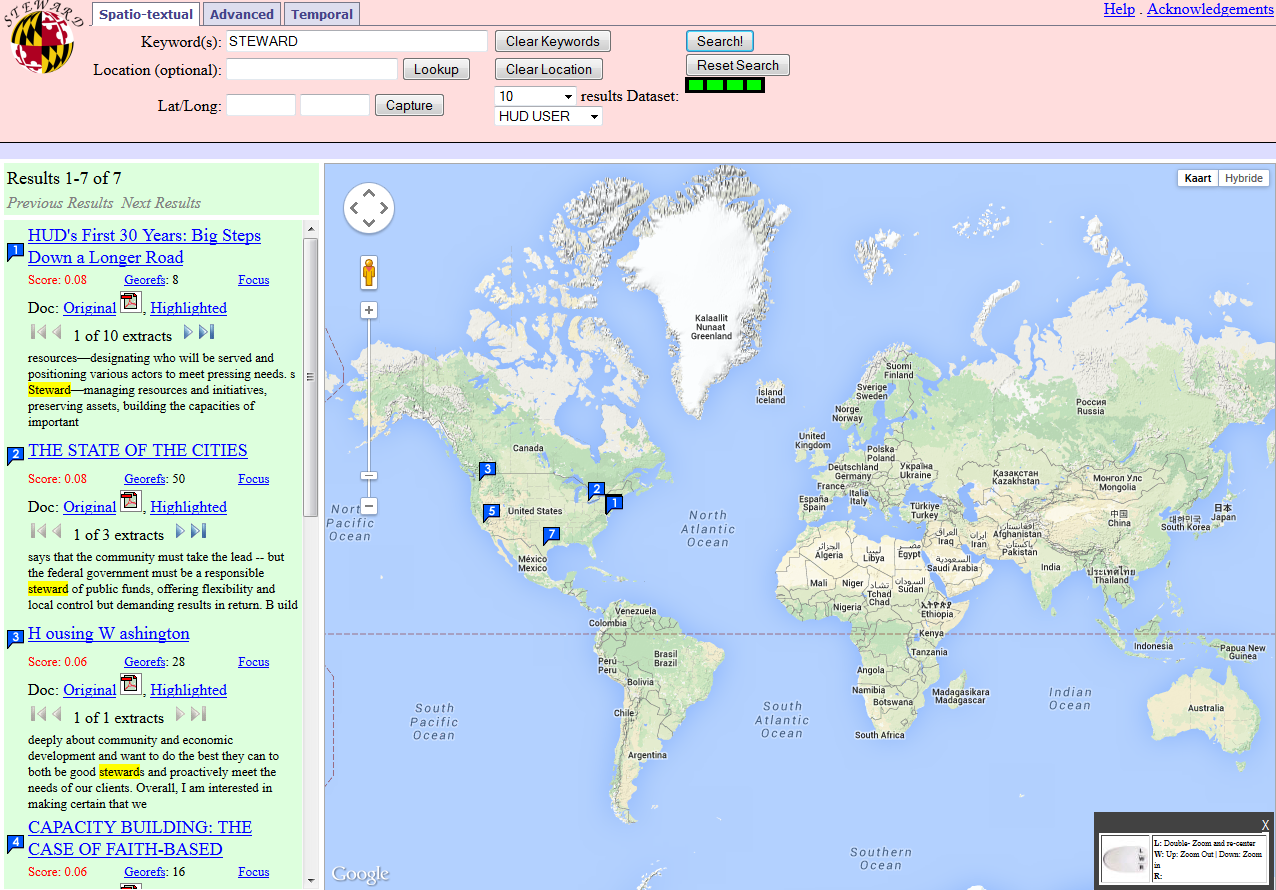
\includegraphics[scale=0.3]{./img/STEWARD.png}
			\caption{STEWARD User Interface}
		\end{figure}
		\\[0.5cm]
		Het STEWARD systeem kan gebruikt worden voor een aantal verschillende toepassingen. Bijvoorbeeld als zoekmachine voor het "hidden web"\footnote{http://en.wikipedia.org/wiki/Deep\_Web}, waar een normale zoekmachine, welke gebruik maakt van een pagerank algoritme\footnote{http://en.wikipedia.org/wiki/PageRank}, niet zal werken door het gebrek aan links naar de documenten. Ook kan er gezocht worden op nieuws, dit gaat nog wel aan de hand van een onderwerp (met eventueel een locatie). De resultaten worden vervolgens op een kaart weer gegeven zodat de gebruiker gemakkelijk kan zien wat de geografische locatie van het artikel is. Daarnaast kan het systeem gebruikt worden als een monitoring systeem voor ziektes, en het verzamelen van touristische, historische en recreationele informatie over een stad of gebied.
	\section{NewsStand: A New View on News \cite{NewsStand2008}}
		Nieuws artikelen bevatten heel veel (implicite) geografische informatie, die niet altijd duidelijk is voor de lezer. Door dit inzichtelijk te maken wordt het begrip van nieuws vergroot. NewsStand doet dit door RSS feeds \cite{RSS} in de gaten te houden. Voor elk artikel wordt de geografische inhoud ge"extraheerd door gebruik te maken van een geotagger, de artikelen worden vervolgens geclusterd. Door in te zoomen op de kaart kunnen gebruikers nieuwsberichten vinden, afhankelijk van hoe ver een gebruiker ingezoomd is worden verschillende nieuwsberichten getoond.
		\\[0.5cm]
		In het artikel wordt besproken waarom een dergelijk systeem nuttig is, en hoe dit systeem is opgebouwd.
	\section{Reading News with Maps by Exploiting Spatial Synonyms \cite{RNwMbESS}}
		Dit artikel uit oktober 2014 is het vervolg op \textit{NewsStand: A New View on News} uit november 2008. De architectuur van NewsStand\footnote{http://newsstand.umiacs.umd.edu/web/} wordt ook in dit artikel weer besproken, net als het proces van het geotaggen en de problemen waar hier rekening mee gehouden moeten worden.
		\\[0.5cm]
		In de toekomst willen zij deze tool uitbreiden zodat er naast tekst ook gezocht kan worden op foto's, videos en audio. Ook willen ze andere soorten nieuwsbronnen gaan gebruiken zoals Twitter.
		\begin{figure}[!htb]
			\centering
			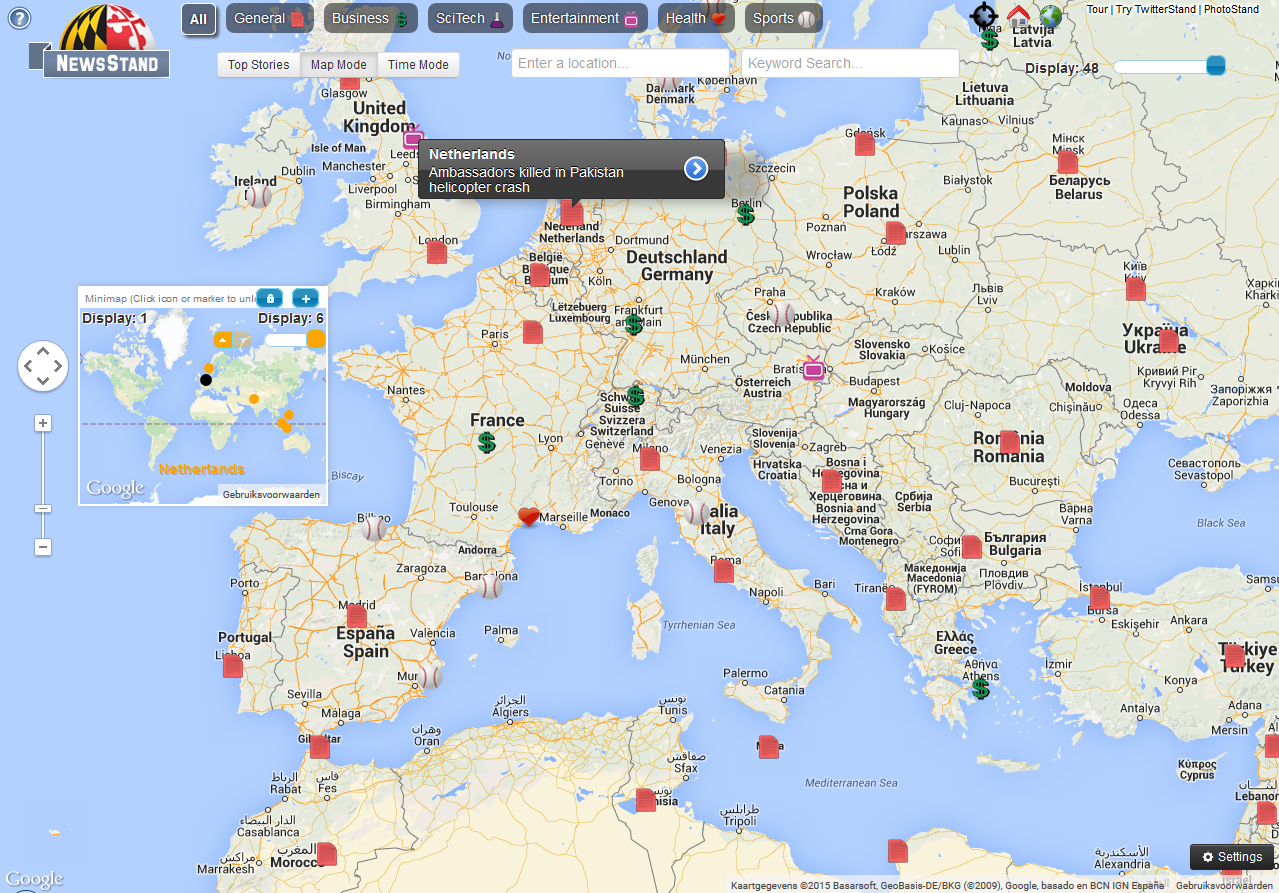
\includegraphics[scale=0.3]{./img/NewsStand.png}
			\caption{NewsStand User Interface}
		\end{figure}
\chapter{Ontwerp}
	In dit hoofdstuk zullen de gemaakte ontwerpkeuzes besproken worden. Ook zullen er twee voorstellen gedaan worden voor de implementatie van een applicatie om nieuws te zoeken aan de hand van een geografische locatie.
	\section{Web applicatie of standalone/desktop applicatie?}
		Een dergelijke applicatie kan ge"implementeerd worden als web applicatie of standalone applicatie. In deze sectie zullen we beide opties bespreken en een keuze tussen deze twee maken.
		\subsection{Web applicatie}
			Een web applicatie is een applicatie die voor gebruikers beschikbaar is via een webserver. Deze server is vaak bereikbaar via het internet maar het is ook mogelijk om dit via intranet te doen. De gebruiker kan via een client programma, zoals een webbrowser, gebruik maken van een dergelijke applicatie.
		\subsection{Standalone/desktop applicatie}
			Een standalone of desktop applicatie is een programma waarbij vooraf bepaald is welke taken uitgevoerd kunnen worden. Vaak zijn dergelijke programma's beschikbaar vanaf een lokale schijf in de computer van een gebruiker en hebben deze programma's in principe geen internet/netwerk nodig om te kunnen functioneren.
		\subsection{Web applicatie vs. standalone/desktop applicatie}
			Om te kunnen beslissen of we beter een web applicatie of een standalone/desktop applicatie kunnen gebruiken moeten we eerst weten welke aspecten van belang zijn bij een dergelijke applicatie. Dat zijn:
			\begin{itemize}
				\item Beschikbaar voor iedereen
				\item Portabiliteit, niet afhankelijk zijn van een besturingssysteem
				\item Privacy
				\item Toegang tot recent nieuws
			\end{itemize}
			Nu we weten welke aspecten belangrijk zijn kunnen we naar de voordelen van zowel web applicaties als standalone/desktop applicaties kijken om vervolgens een keuze te maken.\\[0.5cm]
			\textbf{Voordelen web applicatie}
			\begin{itemize}
				\item Snel voor iedereen toegankelijk
				\item Overal beschikbaar (waar internet is)
				\item Geen onderhoud (updates installeren) voor de gebruiker
				\item Niet afhankelijk van besturingssysteem
			\end{itemize}
			\textbf{Voordelen standalone/desktop applicatie}
			\begin{itemize}
				\item Veiliger, er wordt geen privacy gevoelige data over het netwerk verstuurd
				\item Lagere kosten voor de gebruiker op de lange termijn
				\item Geen internet verbinding nodig
				\item Sneller
				\item Mogelijkheid om backups van data te maken
			\end{itemize}
			Hier uit blijkt dat een web applicatie het beste aansluit bij de aspecten die voor ons van belang zijn. Wel moet er goed gekeken worden naar de privacy bij de ontwikkeling van een dergelijke applicatie, dit omdat we gegevens over een netwerk versturen. Om te voorkomen dat andere mensen mee kijken met ons netwerk verkeer kunnen we gebruik maken van beveiligde protocollen.
	\section{Server}
		Zoals in de voorgaande sectie beschreven is er gekozen voor een web applicatie. Hiervoor moet een server ge"implementeerd worden, in deze sectie worden de ontwerp keuzes besproken die betrekking hebben op deze webserver.
		\section{Python, PHP of Ruby on Rails}
			Drie mogelijke talen om een web applicatie mee te ontwikkelen zijn PHP\footnote{http://php.net/}, Ruby\footnote{https://www.ruby-lang.org/en/} en Python\footnote{https://www.python.org/}, van deze talen is PHP de meest gebruikte. In figuur \ref{fig:phpvspython} wordt een vergelijking gemaakt tussen de drie talen. In figuur \ref{fig:phpvspython3} is te zien dat PHP verreweg de meest gebruikte taal is.
			\begin{figure}[!htb]
				\centering
				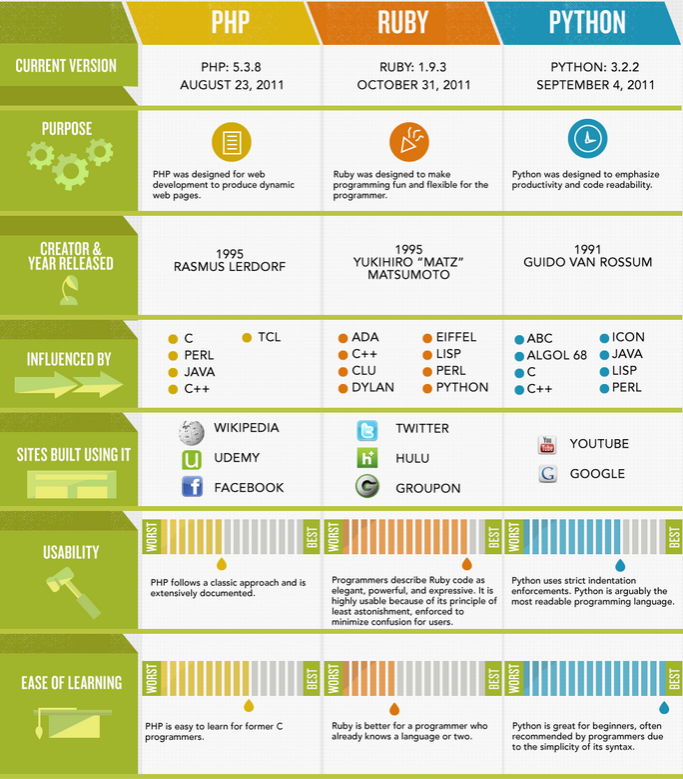
\includegraphics[scale=0.9]{./img/phpvspython.png}
				\caption{Vergelijking PHP, Ruby en Python, bron: Udemy}
				\label{fig:phpvspython}
			\end{figure} 
			\begin{figure}[!htb]
				\centering
				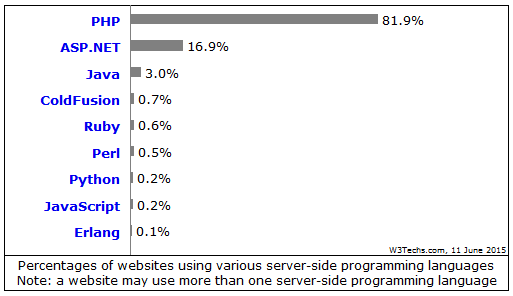
\includegraphics[scale=0.9]{./img/phpvspython3.png}
				\caption{Vergelijking PHP, Ruby en Python, bron: http://w3techs.com}
				\label{fig:phpvspython3}
			\end{figure} 
			\subsection{PHP}
				PHP, \textit{P}HP: \textit{H}ypertext \textit{P}reprocessor, is een scripttaal waarmee dynamische webpagina's ontwikkeld kunnen worden. De taal is in 1994 ontworpen door Rasmus Lerdorf, en ge"inspireerd door Perl\footnote{https://www.perl.org/}. Tegenwoordig is dit de meest gebruikte taal om web applicaties mee te ontwikkelen. 
			\subsection{Ruby}
				Ruby is een programmeertaal waarmee eenvoudig en snel objectge"orienteerd geprogrammeerd kan worden, de taal is in 1995 gepubliceerd door Yukihiro Matsumoto. Sinds 2004 is Ruby on Rails beschikbaar, dit is een open source web applicatie-framework geschreven in Ruby. 
			\subsection{Python}
				Python is een in 1991 verschenen programmeertaal, de taal is door Guido van Rossum ontwikkeld. Het is een van de eenvoudigste talen om te leren en omdat het erg op psuedo code lijkt is het meestal ook goed te lezen en te begrijpen voor mensen die zelf niet kunnen programmeren.
				\\[0.5cm]
			Voor dit project is gekozen om gebruik te maken van Python, in combinatie met CherryPy en Cheetah. We hebben hier voor gekozen omdat het een stuk sneller is dan PHP wat betreft run time en het aantal regels code nagenoeg gelijk is aan het aantal dat bij PHP nodig zou zijn, zie figuur \ref{fig:phpvspython2}. Hierbij is er ook rekening mee gehouden dat met Python ook standalone applicaties gemaakt kunnen worden, iets wat met PHP (bijna) niet mogelijk is. Op deze manier kan een groot deel van de code direct gebruikt worden als er behoefte is aan een standalone/desktop applicatie.
			\begin{figure}[!htb]
				\centering
				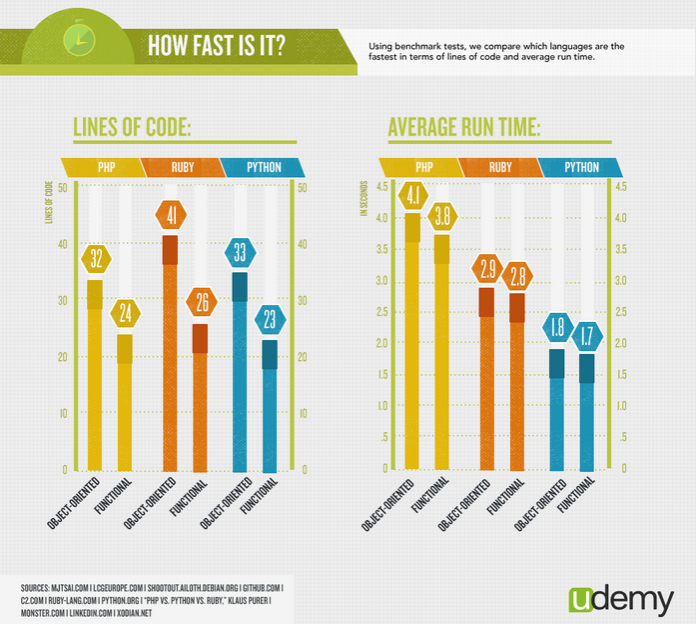
\includegraphics[scale=0.9]{./img/phpvspython2.png}
				\caption{Vergelijking snelheid PHP, Ruby en Python, bron: Udemy}
				\label{fig:phpvspython2}
			\end{figure}
		\subsection{CherryPy}
			CherryPy \cite{CherryPy} is een open-source (BSD license\footnote{https://en.wikipedia.org/wiki/BSD\_licenses}) minimalistisch Python Web Framework, hiermee is het mogelijk om web applicaties te maken op (bijna) de zelfde manier als een objectge"orienteerd Python programma. Het resultaat hiervan is dat er minder code nodig is en het ontwikkelen van een web applicatie minder tijd kost.
			\\[0.5cm]
			Inmiddels bestaat CherryPy al meer dan tien jaar en heeft het bewezen zeer snel en stabiel te zijn. Het wordt gebruikt bij veel websites, van kleine simpele sites tot zeer veel eisende applicaties.
			\\[0.5cm]
			Een voorbeeld van een simpele website met CherryPy is het volgende:
			\begin{verbatim}
			import cherrypy
			
			class HelloWorld(object):
			@cherrypy.expose
			def index(self):
			    return "Hello world!"
			
			if __name__ == '__main__':
			    cherrypy.quickstart(HelloWorld())
			\end{verbatim}
			Deze code start een webserver met de standaard configuratie en print de tekst ``Hello World!'' op de pagina. Het is ook mogelijk om een eigen configuratie voor de server te gebruiken, zoals hier onder te zien is, hierin is \textit{cherry\_conf} een Python dictionary\footnote{https://docs.python.org/2/tutorial/datastructures.html\#dictionaries}. Op deze manier kan er bijvoorbeeld handmatig bepaald worden op welk IP adres de server te vinden is en welke poort, standaard $8080$, er gebruikt wordt. 
			\begin{verbatim}
			cherrypy.quickstart(HelloWorld(), config = cherry_conf)
			\end{verbatim}
			In plaats van een simpele tekst op het scherm willen we graag een complete HTML pagina terug geven, dit doen we door gebruik te maken van Cheetah.
		\subsection{Cheetah}
			Cheetah \cite{Cheetah} of Cheetah Template is een template engine die gebruik maakt van Python. Het kan apart gebruikt worden of in combinatie met andere tools en frameworks, zoals bijvoorbeeld CherryPy. Over het algemeen wordt het gebruikt voor server-side scripting en het genereren van dynamische webpagina's. Een simpel voorbeeld is hier onder te zien, deze Cheetah template genereerd een HTML pagina met daarop een tabel waarin voor elke client een regel wordt gemaakt met de achternaam, voornaam en een link naar het emailadres.
			\begin{verbatim}
			<html>
			    <head>
			        <title>
			            $title
			        </title>
			    </head>
			    <body>
			        <table>
			        #for $client in $clients
			            <tr>
			                <td>
			                    $client.surname, $client.firstname
			                </td>
			                <td>
			                    <a href="mailto:$client.email">$client.email</a>
			                </td>
			            </tr>
			        #end for
			        </table>
			    </body>
			</html>
			\end{verbatim}
			Voor dit project gebruiken we Cheetah om een template te maken van de User Interface.
		\subsection{JSON}
			JSON \cite{JSON} staat voor Javascript Object Notation, het is een simpel formaat voor gegevens uitwisseling. Het is gemakkelijk door computers te verwerken en goed leesbaar voor mensen. Nagenoeg alle programmeertalen ondersteunen JSON, zo ook Python. Hier onder volgt een voorbeeld van JSON.
			\begin{verbatim}
			[
			    { 
			        "Naam": "JSON",
			        "Type": "Gegevensuitwisselingsformaat",
			        "isProgrammeertaal": false,
			        "Zie ook": [ "XML", "ASN.1" ] 
			    },
			    { 
			        "Naam": "JavaScript",
			        "Type": "Programmeertaal",
			        "isProgrammeertaal": true,
			        "Jaar": 1995 
			    } 
			]
			\end{verbatim}
			Wij gebruiken JSON om de lijst met steden en landen terug te sturen naar de client en ook de nieuwsberichten worden als JSON object opgevraagd. 
		\subsection{AJAX}
			AJAX \cite{AJAX}, \textit{A}synchronous \textit{J}avaScript \textit{A}nd \textit{X}ML, wordt gebruikt bij de ontwikkeling van interactieve webpagina's, waarbij asynchroon gegevens van de server worden opgehaald. Dat wil zeggen dat we niet de hele pagina hoeven te vernieuwen als we bijvoorbeeld een andere afbeelding willen laden. Bij dit project maken we gebruik van AJAX om de co"ordinaten van het middelpunt en de straal van het geselecteerde gebied naar de server te verstruren. Ook het uitvoeren van zoekopdrachten voor nieuwsberichten gaat via AJAX. Hiervoor gebruiken we de standaard functies die voor AJAX in JQuery \cite{JQuery} ge"implementeerd zijn.
		\subsection{JQuery}
		JQuery is een JavaScript framework waarmee dynamische en interactieve websites gemaakt kunnen worden. Hiermee kunnen we de DOM en CSS van websites aanpassen zonder de bron code aan te moeten passen, op deze manier kunnen we bijvoorbeeld een tabel uitbreiden of de lay-out aanpassen voor \'e\'en gebruiker. Daarnaast heeft JQuery ook ondersteuning voor AJAX. JQuery is beschikbaar onder de MIT-licentie en de GNU General Public License.
	\section{Database}
		\label{sec:db}
		Voor de database hebben we gekozen voor een SQLite \cite{SQLite} database. SQLite is een software pakket wat een SQL database engine implementeerd, maar in tegenstelling tot bijvoorbeeld MySQL is hier geen client/server systeem voor nodig. Bij SQLite wordt de database in \'e\'en bestand op de schijf opgeslagen.
		\\[0.5cm]
		Omdat SQLite standaard geen ondersteuning heeft voor veel wiskundige functies zijn deze toegevoegd via een extensie. Hiervoor wordt het bestand \textit{extension-functions.c}\footnote{https://www.sqlite.org/contrib} gebruikt, hierin zijn functies als \textit{cos} en \textit{sin} ge"implementeerd.
	\section{Geografische informatie}
		\label{sec:geo_info}
		Voor de geografische informatie, de steden met hun breedtegraad en lengtegraad, populatie en landen is gekeken naar de mogelijkheid om dit via Google Maps \cite{MapsJS} te doen. Hoewel dit in theorie mogelijk is, is dit in praktijk geen goede optie. We zouden dan alle steden die in Google Maps te vinden zijn eerst moeten downloaden en opslaan in een database voordat we kunnen gaan berekenen of ze in het geselecteerde gebied liggen.
		\\[0.5cm]
		Een andere mogelijkheid waar naar gekeken is, is om gebruik te maken van Wolfram Alpha \cite{Wolf}, hiermee is het mogelijk om de afstand tussen twee steden op aarde te berkenen. Wel moeten we dan zelf de breedtegraad en lengtegraad van het start en eind punt hebben, we kunnen hiermee dus geen steden zoeken.
		\\[0.5cm]
		GeoNames \cite{Geonames} is een database waar (vrijwel) alle steden op de wereld in te vinden zijn. De database bevat heel veel informatie waarvan, voor ons, vooral de naam van de stad, de populatie, de breedtegraad en lengtegraad en het land waar de stad in ligt interessant zijn. Voor landen en steden zijn ook alternatieve namen, in andere talen dan Engels, te vinden in de database. Daarnaast zijn ook zee"en, oceanen, meren, bergen etc. op te zoeken. Voor dit project is alleen gekeken naar steden en landen maar voor een toekomstig onderzoek zijn dit interessante opties.
		\\[0.5cm]
		De database is via een API te benaderen of te downloaden als tekstbestand. Bij dit project is voor het laatste gekozen om het netwerk verkeer zo beperkt mogelijk te houden en om te zorgen dat de data altijd beschikbaar is. Omdat een tekstbestand niet effici"ent te door zoeken is schrijven we de data naar onze eigen SQLite database.
		\\[0.5cm]
		Tijdens de ontwikkeling van de applicatie bleek dat voor een deel van de steden, $32480$ van de $144573$, geen populatie beschikbaar is. Omdat we bij het algoritme voor de gebiedsrepresentatie kijken wat de grootste stad in een gebied is en dit niet mogelijk is met twee of meer steden waarvan de populatie gelijk is aan $0$ worden deze steden uitgesloten tijdens de selectie. In sectie \ref{sec:citiespop} wordt een voorstel gedaan hoe dit opgelost zou kunnen worden zodat deze steden wel gebruikt kunnen worden. Een ander probleem wat tijdens de implementatie boven kwam is dat een aantal grote steden, zoals Londen en Parijs, in meerdere delen in de database opgeslagen zijn. Ook dit kan voor problemen zorgen bij het algoritme voor de gebiedsrepresentatie. Een oplossing hiervoor is te vinden in sectie \ref{sec:multcities}.
	\section{Nieuwsbronnen}
		Voor de ontwikkeling van de applicatie is gekeken naar meerdere nieuwsbronnen. Hier zullen we een aantal van deze bronnen bespreken.
		\subsection{Google News}
			Google News \cite{NewsAPI} is een zoekmachine van Google om nieuws berichten te doorzoeken. De titles, eerste alinea's en afbeeldingen van nieuwsberichten op het internet worden verzameld en kunnen aan de hand van keywords worden doorzocht. Voor deze dienst is een API beschikbaar maar deze wordt sinds 26 mei 2011 niet meer ondersteund. Er kan nog wel gebruik van gemaakt worden, maar de API wordt niet meer bijgewerkt. Daarnaast is er geen garantie dat de API goed werkt. 
		\subsection{BING News}
			BING News \cite{BINGNews} is een vergelijkbare zoekmachine van Microsoft. Ook hier is een API voor beschikbaar, welke nog wel ondersteund wordt. Per maand kunnen hier gratis $5000$ zoekopdrachten mee uitgevoerd worden, mocht er meer nodig zijn dan is dit mogelijk tegen betaling.
		\subsection{Overig}
			Naast Google News en BING News hebben we nog naar een aantal andere optie gekeken.
			\subsubsection{Yahoo News Service}
				Ook deze zoekmachine is te vergelijken met Google News en BING News. Hier voor is ook een API \cite{YahooNews} beschikbaar, deze is echter alleen te gebruiken tegen betaling. Voor dit project is dat niet haalbaar maar mogelijk dat dit in de toekomst een interessante optie is.
			\subsubsection{FAROO}
				FAROO \cite{Faroo} is een alternatief voor de hierboven genoemde opties. Het is een gratis zoek API waarbij tot 1 miljoen zoekopdrachten per maand gedaan kunnen worden. 
			\subsubsection{Lokaal nieuws}
				Een hele interessante optie is om lokale nieuws sites en kranten te zoeken bij het geselecteerde gebied. Vooral voor kleinere gebieden, zal dit nuttige resultaten op kunnen leveren. in sectie \ref{sec:localnews} gaan we hier dieper op in.
	\section{Zoeken naar nieuws}
		Het zoeken naar nieuws gaat via de BING API \cite{BINGNews}. Hiermee is het mogelijk om gratis $5000$ zoekopdrachten per maand uit te voeren, tegen betaling kunnen er meer zoekopdrachten uitgevoerd worden. We kunnen het beste zoeken aan de hand van de naam van een stad en het land waar deze stad in te vinden is. Dit is nodig omdat wanneer we alleen op de naam van een stad zoeken, en deze stad komt in meerdere landen voor, we ook resultaten uit andere landen krijgen die niks met het zoek gebied te maken hebben. Bijvoorbeeld Willemstad in Noord Brabant, Nederland en Willemstad in Cura\c{c}ao. Voor dit project maken we hier geen gebruik van omdat als we een zoekopdracht uitvoeren met ``Willemstad, Nederland'' we ook nieuws terug krijgen waar alleen ``Nederland'' in vermeldt wordt, hier is nog geen goede oplossing voor gevonden. 
		\subsection{Client side of server side?}
			Het zoeken naar nieuws kan zowel client side als server side gebeuren.
			Het zoeken van nieuws door de server heeft als voordeel dat het mogelijk is om een cache aan te leggen, van nieuws wat bij een stad hoort. Daarbij komt dat de sleutel van de BING API niet beschikbaar is voor de gebruiker en dus niet misbruikt kan worden. Het is echter toch wenselijk om dit client side te doen omdat we op deze manier de netwerk en server belasting kunnen verspreiden. 
	\section{Ideaal ontwerp}
		In deze sectie beschrijven we een voorstel hoe een dergelijke applicatie eigenlijk zou moeten. Helaas is het vooral door gebrek aan tijd en middelen niet mogelijk om het op deze manier te doen. 
		\\[0.5cm]
		Zoals eerder gezegd heeft het zoeken naar nieuws door de server een aantal voordelen. Dit zoeken zou dan ook niet meer via bijvoorbeeld BING News gaan, een betere optie is om gebruik te maken van RSS feeds \cite{RSS}.
		\subsubsection{RSS feeds}
			RSS staat voor \textit{R}ich \textit{S}ite \textit{S}ummary, maar ook vaak \textit{R}eally \textit{S}imple \textit{S}yndication genoemd, het is een eenvoudige manier om op de hoogte te blijven van bijvoorbeeld het laatste nieuws. Het is gemaakt zodat we niet zelf alle sites hoeven te bezoeken waarvan we op de hoogte willen blijven van de nieuwste berichten. In plaats daarvan kunnen we de RSS feed in de gaten houden, de nieuwste berichten komen hier automatisch op te staan.
			\\[0.5cm]
		Met een achtergrond proces op de server kunnen deze RSS feeds in de gaten gehouden worden en zodra er een nieuw nieuws bericht beschikbaar is wordt deze gedownload. Eenmaal gedownload moet een bericht geanalyseerd worden om te bepalen bij welke stad het bericht hoort. Nieuwsberichten die geanalyseerd zijn worden opgeslagen in een database, met bijvoorbeeld de stad en het land waar het bericht bij hoort, een link naar het bericht en de tijd dat het nieuwsbericht gepubliceerd is. Deze tijd kan gebruikt worden om te bepalen of het nog een actueel bericht is.
		\\[0.5cm]
		Met de hier beschreven methode verstuurt de client alleen nog het middelpunt en de straal van de op de kaart gemaakte selectie. De server doet de rest van het werk, dat wil zeggen het zoeken naar steden die bij het geslecteerde gebied horen, het zoeken naar nieuws dat bij deze steden horen en vervolgens deze lijst met nieuwsberichten terug sturen naar de client. Op deze manier is het ook eenvoudig om nieuwsbronnen toe te voegen, we hoeven alleen de RSS feed van de bron in de gaten te houden.
	\section{Samenvatting}
		In dit hoofdstuk hebben we gezien hoe we een applicatie om nieuws te zoeken aan de hand van een locatie kunnen opbouwen. Er is gekozen om een web applicatie te ontwikkelen waarbij de server verantwoordelijk is voor de selectie van de steden die in een gebied liggen. De client zoekt vervolgens naar nieuws. \\[0.5cm]
		Ook hebben we gezien welke nieuwsbron we kunnen gebruiken, namelijk BING News. Daarnaast hebben we gekeken naar andere mogelijke nieuwsbronnen zoals Google News, Faroo en Yahoo News Service.
		\\[0.5cm]
		Met dit hoofdstuk hebben we de vraag \textit{Welke nieuwsbronnen kunnen we gebruiken?} beantwoord. Ook is er een begin gemaakt met het antwoord op 
		de vraag \textit{Hoe implementeren we een dergelijke applicatie?}, hiermee zullen we verder gaan in het volgende hoofdstuk.
\chapter{Implementatie}
	Hier onder zullen we de implementatie van de hiervoor gemaakte ontwerpkeuzes beschrijven.
	\begin{figure}[!htb]
		\label{fig:arch}
		\centering
		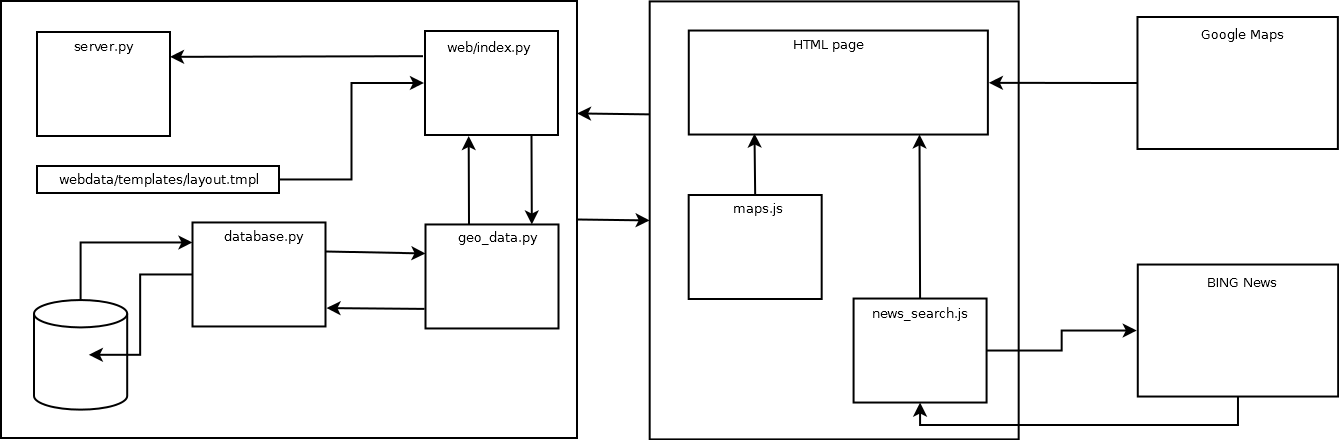
\includegraphics[scale=0.3]{./img/architecture.png}
		\caption{Architectuur}
	\end{figure}
	De code en de installatie van de server zijn uitgebreider toegelicht in bijlage \ref{app:install}.
	\section{Server en database}
		\subsection{Server}
		De server is geschreven in Python en maakt gebruik van CherryPy en Cheetah. In principe is de server ge"implementeerd als webserver maar zou ook gebruikt kunnen worden als API \cite{API} voor een andere applicatie.
		
		\subsubsection{Webserver}
		Op de webserver draait \'e\'en pagina, \textit{web/index.py}, de template met daarin alle HTML voor deze pagina is te vinden in \textit{webdata/templats/layout.tmpl}.
		\\[0.5cm]
		Wanneer \textit{web/index.py} een HTTP GET request \cite{HTTP} krijgt wordt de HTML uit deze template terug gestuurd naar de gebruiker.
		\\[0.5cm]
		Zodra een gebruiker een gebied op de kaart selecteerd wordt er een HTTP POST request door de client naar de server gestuurd. De door de client opgestuurde data, de breedtegraad en lengtegraad van het middelpunt en straal van het gebied, wordt gecontroleerd en de steden die bij dit gebied horen worden opgezocht. Deze steden worden in een JSON object terug gestuurd naar de client.
		\subsubsection{API}
		Om de server te gebruiken als API voor een andere applicatie maken we alleen gebruik van de HTTP POST request \cite{HTTP}, hierin sturen we de breedtegraad en lengtegraad van het middelpunt en de straal van het gebied. Vervolgens krijgen we een JSON object terug met de steden die dit gebied representeren welke we verder kunnen verwerken voor onze applicatie.
		\begin{verbatim}
		POST / HTTP/1.1
		Host: 192.168.0.18:8080	
		User-Agent: Mozilla/5.0 (Windows NT 6.1; WOW64; rv:38.0) Gecko/20100101 Firefox/38.0
		Accept: text/html,application/xhtml+xml,application/xml;q=0.9,*/*;q=0.8
		Accept-Language: nl,en-US;q=0.7,en;q=0.3
		Accept-Encoding: gzip, deflate
		Content-Type: application/x-www-form-urlencoded; charset=UTF-8
		Referer: http://192.168.0.18:8080/
		Content-Length: 68
		Cookie: session_id=5c6f93c64ae57b5c0433122dac235099a1dcb4d5
		Connection: keep-alive
		Pragma: no-cache
		Cache-Control: no-cache
		
		lat=52.3740300&lon=4.8896900&radius=50.0
		\end{verbatim}
		Als we het hier bovenstaande HTTP POST request naar de server sturen die op IP adres $192.168.0.18:8080$ draait krijgen we een lijst met steden terug die binnen $50km$ van Amsterdam liggen.
		\subsection{Database}
			Zoals uitgelegd in sectie \ref{sec:db} maken we gebruik van een SQLite database, Python heeft hier ondersteuning voor via de \textit{sqlite3} \cite{sqlite3} module.\\[0.5cm]
			De database, figuur \ref{fig:db} bevat twee tabellen, \textit{cities} en \textit{countries}. De \textit{cities} tabel bevat alle steden, elke stad in de tabel heeft een uniek ID, een naam, een aantal inwoners, een code voor het land waarin deze stad ligt en de co\"ordinaten, breedtegraad en lengtegraad, van de stad. De landcode verwijst naar de tabel \textit{countries}, hiermee kan de naam van het land waarin de stad ligt opgezocht worden. \\[0.5cm]
			De tweede tabel in de database is de \textit{countries} tabel,  met velden voor de naam en de code van het land.
			\begin{figure}[!htb]
				\label{fig:db}
				\centering
				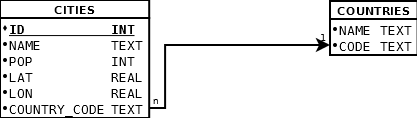
\includegraphics[scale=0.6]{./img/database.png}
				\caption{Database}
			\end{figure}
			\subsubsection{database.py}
			Bij een SQL query is een groot deel van de query vast, bij bijvoorbeeld een SELECT query veranderen alleen de naam van de tabel en de velden die we willen selecteren.
\begin{verbatim}
SELECT x, y, z FROM table;
\end{verbatim}
			Om niet elke keer een hele query te moeten maken staan er in dit bestand functies waarbij we aan kunnen geven welke velden van welke tabel we willen selecteren, de functie maakt de SQL query en voert deze ook direct uit. Er zijn functies voor het selecteren, toevoegen, updaten en verwijderen van entries in de database. Daarnaast zijn er ook functies voor het maken en verwijderen van tabellen.
		\subsection{geo\_data.py}
		In dit Python bestand staan functies voor het downloaden van de geografische informatie van \textit{geonames.org}. Deze informatie is beschikbaar in een tekst bestand, omdat dit niet effici"ent is als er gekeken moet worden welke steden er in een gebied liggen is er een functie om deze data naar de database te schrijven. In principe wordt dit alleen de eerste keer gedaan, maar mocht het nodig zijn kan de database opnieuw opgebouwd worden.\\[0.5cm]
		Behalve de functies om de database te downloaden en op te bouwen zijn er ook functies om de steden te zoeken en een algoritme om te bepalen welke steden het gebied representeren hier ge"implementeerd.
	\section{Welke steden liggen in het geselecteerde gebied?}
		Een door de gebruiker op de kaart geselecteerd gebied wordt weergegeven door de co\"ordinaten van het middelpunt (breedtegraad\footnote{http://en.wikipedia.org/wiki/Latitude} en lengtegraad\footnote{http://en.wikipedia.org/wiki/Longitude}) en de straal van de cirkel (het gebied) in kilometers.
		\\[0.5cm]
		Om te berekenen welke steden binnen dit gebied liggen moet de afstand van het middelpunt tot een stad berekend worden. Is deze afstand kleiner dan of gelijk aan de straal van het geselecteerde gebied, dan ligt de stad in het gebied.
		\\[0.5cm]
		Voor het berekenen van de afstand tussen twee punten $P_1(lat_1, lon_1)$ en $P_2(lat_2, lon_2)$ op een bol, zoals de aarde,  kan geen gebruik gemaakt worden van de stelling van Pythagoras \cite{Pytha} omdat deze stelling uit gaat van een plat vlak. Om de afstand tussen twee punten op een bol te berekenen kan gebruik gemaakt worden van bijvoorbeeld de \textit{spherical law of cosines} \cite{spherical} of de \textit{haversine formule} \cite{haversine}. De \textit{haversine formule} is vooral voor kleine afstanden nauwkeuriger, met deze formule kunnen afstanden tot ongeveer \'e\'en meter nauwkeurig berekend worden. Bij de \textit{spherical law of cosines} is de maximale fout een paar meter. Om deze reden wordt de \textit{haversine formule} meer gebruikt bij navigatie, voor dit project is een fout van een paar meter echter niet belangrijk. Er is daarom gekozen voor de \textit{spherical law of cosines}.
		\\[0.5cm]
		$distance = \arccos(\sin(lat_1) \cdot \sin(lat_2) + \cos(lat_1) \cdot \cos(lat_2) \cdot(lon_1 - lon_2)) \cdot R$
		\\[0.5cm]
		Hierin zijn $(lat_1, lon_1)$ de co"ordinaten van het startpunt, in dit geval het middelpunt van het geselecteerde gebied, en $(lat_2, lon_2)$ de co"ordinaten van het tweede punt waarvoor we de afstand tot het start punt willen berekenen. Deze co"ordinaten worden door de client in graden door gestuurd en moeten eerst omgezet worden naar radialen om in deze formule gebruikt te kunnen worden. $R$ is de straal van de bol waarop beide punten liggen, in dit geval de aarde $ 	\Rightarrow R = 6371km$.
		\\[0.5cm]
		Met deze formule zou meteen een \textit{SQL \cite{SQL} query} geconstrueerd kunnen worden.
\begin{verbatim}
SELECT
    cities.NAME, cities.LAT, cities.LON, cities.POP
FROM 
    cities 
WHERE 
    acos(sin(lat) * sin(cities.lat) + cos(lat) * cos(cities.lat) * cos(lon - cities.lon)) * 
    6371 <= radius;
\end{verbatim}
		Deze query geeft als resultaat een lijst met steden die binnen het door de gebruiker geselecteerde gebied liggen. Voor elke stad wordt de naam, populatie, breedtegraad en lengtegraad terug gegeven.
		\\[0.5cm]
		Nadeel van deze query is echter dat voor alle steden in de database berekend moet worden of de afstand tot het middelpunt van het geselecteerde gebied kleiner dan of gelijk is aan de straal van het gebied. Dit kost veel tijd, om dit te versnellen selecteren we alleen kandidaat steden waar we vervolgens de berekening op uit gaan voeren. Door de minimale en maximale breedtegraad en lengtegraad te berekenen kunnen we al een heleboel steden uitsluiten die sowieso buiten het geselecteerde gebied liggen.
		\subsubsection{Berekenen minimale en maximale breedtegraad}
		Als je van een punt $A$ naar een punt $B$ op een cirkel gaat kun je de hoek, $r$, tussen deze twee punten berekenen. Lengtecirkels (meridianen)\footnote{http://en.wikipedia.org/wiki/Meridian\_(geography)} zijn dergelijke cirkles op aarde met een straal van $R = 6371km$. Je kan dus over een meridiaan verplaatsen, dat wil zeggen de lengtegraad blijft constant, en simpelweg $r$ aftrekken/optellen bij de breedtegraad van het middelpunte van het geselecteerde gebied om de minimale en maximale breedtegraad te krijgen.
		\\[0.5cm]
		$lat_{min} = lat - r$ \\
		$lat_{max} = lat + r$
		\\[0.5cm]
		$r$ hangt af van de afstand tussen de twee punten en de straal $R$ van de aarde. De afstand tussen de twee punten stellen we gelijk aan de maximale afstand dat een stad nog in het geselecteerde gebied ligt, dat is de straal van het gebied.
		\\[0.5cm]
		$r = \frac{max. distance}{R} = \frac{radius}{R}$
		\subsubsection{Berekenen minimale en maximale lengtegraad (methode 1)}
		Een door veel applicatie gebruikte benadering om de minimale en maximale lengtegraad te berekenen is een vaste breedtegraad kiezen en de lengtegraad aanpassen. dat betekent dat er over een breedtecirkel \cite{circlelat} bewogen wordt. In deze sectie zullen we aan de hand van een voorbeeld laten zien dat dit geen nauwkeurige resultaten geeft.
		\\[0.5cm]
		Als we over een breedtecirkel bewegen, bewegen we over een zogenaamde kleine cirkel \cite{circlesphere}. Een breedtecirkel op breedtegraad $lat = 1.3963$ heeft een straal $R_{S} = R \cdot \cos(lat) = 6371 \cdot \cos(1.3963) = 1106km$. Een afstand van $1000km$ op deze breedtecirkel komt nu overeen met een hoek $r_{S} = \frac{d}{R_{S}} = \frac{1000}{1106} = 0.9039$ tussen twee punten op deze cirkel. Bij een lengtegraad van $-0.6981$ van het beginpunt komen de minimale en maximale lengtegraad nu op
		\\[0.5cm]
		$lon_{min} = -0.6981 - 0.9039 = -1.6020$\\
		$lon_{max} = -0.6981 + 0.9039 = 0.2058$\\[0.5cm]
		Dit is echter \textbf{niet} de minimale en maximale lengtegraad die we kunnen bereiken door $1000km$ in een willekeurige richting te bewegen vanaf het beginpunt $M = (1.3969, -0.6981)$. Dat komt omdat we ons verplaatsen over een kleine cirkel, afstanden over een kleine cirkel zijn groter dan over een grote cirkel \cite{greatcircle}. Hoewel we dus $1000km$ afgelegd hebben op een kleine cirkel om van $M = (1.3969, -0.6981)$ naar $P_{S} = (1.3969, -1.6020)$ kunnen we ``afsnijden'' op een grote cirkel. Deze afstand is\\[0.5cm]		
		$dist = \arccos(\sin(lat_1) \cdot \sin(lat_2) + \cos(lat_1) \cdot \cos(lat_2) \cdot \cos(lon_1 - lon_2)) \cdot R$\\
		$= \arccos(\sin(1.3963) \cdot \sin(1.3963) + \cos(1.3963) \cdot \cos(1.3963) \cdot \cos(-0.6981 - (-1.6020))) \cdot 6371$\\
		$= 967km$\\[0.5cm]
		We kunnen dus nog $33km$ verder verplaatsen en zitten dan nog steeds binnen het geselecteerde gebied, dat wil zeggen dat we een kleinere en grotere minimale en maximale lengtegraad kunnen bereiken.\\[0.5cm]
		Als we dus gebruik maken van $lon \pm \frac{d}{\cos(lat)}$ als grenzen voor de lengtegraad, sluiten we een aantal plaatsen uit die in werkelijkheid wel in het gebied liggen. Een punt $P = (1.4618, -1.6021)$ ligt buiten de berekende grenzen voor een gebied met middelpunt $M = (1.3969, -0.6981)$ en straal $d = 1000km$  terwijl de afstand van $M$ maar $872km$ is, een fout van meer dan $12\%$.
		\subsubsection{Berekenen minimale en maximale lengtegraad (methode 2)}
		De methode omschreven in de vorige sectie om de minimale en maximale lengtegraad te berekenen werkt dus niet goed. Dit is te zien in figuur \ref{fig:tangentpoints}, de punten op de cirkel met de minimale en maximale lengtegraad $T_1$ en $T_2$ liggen niet op de zelfde breedtecirkel \cite{circlelat} als $M$, het middelpunt van het geselecteerde gebied maar dichter bij de pool.
		\begin{figure}[!htb]
			\centering
			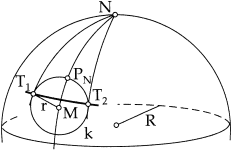
\includegraphics[scale=1.0]{./img/TangentPoints.png}
			\caption{Tangent meridians to the query circle}
			\label{fig:tangentpoints}
		\end{figure}
		In plaats daar van moeten de volgende formules gebruikt worden
		\\[0.5cm]
		$lat_T = \arcsin(\frac{\sin(lat)}{\cos(r)})$\\
		$\Delta lon = \arccos(\frac{\cos(r) - \sin(lat_T) \cdot \sin(lat)}{\cos(lat_T) \cdot \cos(lat)})$ \\
		$= \arcsin(\frac{\sin(r)}{cos(lat)})$
		\\[0.5cm]
		$lon_{min} = lon_{T_1} = lon - \Delta lon$\\
		$lon_{max} = lon_{T_2} = lon + \Delta lon$
		\subsubsection{SQL query}
		Aan de hand van de hierboven berekende minimale en maximale breedtegraad en lengtegraad kunnen we nu een SQL query maken die de berekening, de spherical law of cosines, alleen hoeft uit te voeren op een veel kleiner aantal kandidaat plaatsen.
\begin{verbatim}
SELECT
    cities.NAME, cities.LAT, cities.LON, cities.POP
FROM 
    cities 
WHERE 
        (cities.LAT >= lat_min AND cities.LAT <= lat_max) 
    AND 
        (cities.LON >= lon_min AND cities.LON <= lon_max) 
GROUP BY
    cities.NAME
HAVING
    acos(sin(lat) * sin(cities.LAT) + cos(lat) * cos(cities.LAT) * 
         cos(cities.LON - (lon))) <= radius;
\end{verbatim}
Deze query selecteert de naam, breedtegraad, lengtegraad en populatie voor elke stad die binnen het geselecteerde gebied valt. Eerst worden alle steden geselecteerd waarvoor de breedtegraad en de lengtegraad binnen de minimale en maximale waardes vallen. Vervolgens wordt voor elk van deze kandidaat plaatsen uitgerekend of deze ook echt binnen het geselecteerde gebied liggen. De query is vervolgens aangepast om ook de landen waarin de steden liggen te selecteren. Dit is nodig omdat sommige steden in meerdere landen voorkomen. Doe je dit niet kan het voorkomen dat je nieuws uit een heel ander wereld deel krijgt dan het gebied wat de gebruiker geselecteerd heeft.
\begin{verbatim}
SELECT
    cities.NAME, cities.LAT, cities.LON, cities.POP, countries.NAME
FROM 
    cities, countries 
WHERE
        cities.COUNTRY_CODE = countries.CODE 
    AND
        (cities.LAT >= lat_min AND cities.LAT <= lat_max) 
    AND 
        (cities.LON >= lon_min AND cities.LON <= lon_max) 
GROUP BY
    cities.NAME
HAVING
    acos(sin(lat) * sin(cities.LAT) + cos(lat) * cos(cities.LAT) * 
         cos(cities.LON - (lon))) <= radius;
\end{verbatim}
Omdat een deel van de steden in de database een populatie van $0$ heeft ($32480$ van de $144573$ steden), en het algoritme voor de gebiedsrepresentatie de grootste stad in een gebied moet vinden selecteren we alleen de steden waarvan de populatie \textbf{niet} $0$ is.
\begin{verbatim}
SELECT
    cities.NAME, cities.LAT, cities.LON, cities.POP, countries.NAME
FROM 
    cities, countries 
WHERE
        cities.COUNTRY_CODE = countries.CODE 
    AND
        (cities.LAT >= lat_min AND cities.LAT <= lat_max) 
    AND 
        (cities.LON >= lon_min AND cities.LON <= lon_max)
    AND
        cities.pop != 0
GROUP BY
    cities.NAME
HAVING
    acos(sin(lat) * sin(cities.LAT) + cos(lat) * cos(cities.LAT) * 
         cos(cities.LON - (lon))) <= radius;
\end{verbatim}
	Een voorbeeld van het resultaat als deze SQL query uitgevoerd wordt is het volgende:
	\begin{verbatim}
	[(u'Alkmaar', 0.918595932323124, 0.08287887939312794, 94853, u'Netherlands'), 
	(u'Amsterdam', 0.9140992660382857, 0.08534118990184153, 741636, u'Netherlands'), 
	(u'Beverwijk', 0.9160069109107156, 0.08127893606782473, 37585, u'Netherlands'), 
	(u'Broek in Waterland', 0.9151489070504352,
	...
	 (u'Zaanstad', 0.9154798214766133, 0.08401247074229824, 140085, u'Netherlands')]
	
	\end{verbatim}
	\section{Gebiedsrepresentatie}
		\label{sec:rep}
		Bij het geselecteerde gebied worden vaak honderd of meer, en bij een groot gebied duizenden, steden gevonden die in dit gebied liggen, een voorbeeld is te zien in figuur \ref{fig:without}. Om voor elke stad naar nieuws te zoeken levert evenveel zoekopdrachten als steden op. Dit gaat erg veel tijd in beslag nemen, ongeveer $300ms$ per zoekopdracht, en levert te veel nieuws op. Een dergelijke hoeveelheid nieuws, in de orde van duizenden artikelen, is voor de gebruiker niet te verwerken en draagt niet bij aan een beter begrip van het nieuws en wat er in het gebied gaande is.
		\begin{figure}[!htb]
			\centering
			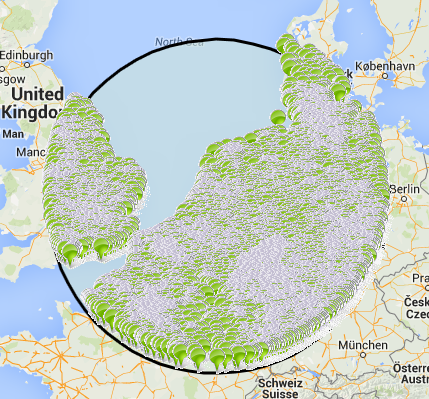
\includegraphics[scale=1.0]{./img/area_wo_algo.png}
			\caption{Alle 12485 steden in een gebied}
			\label{fig:without}
		\end{figure}
		\begin{figure}[!htb]
			\centering
			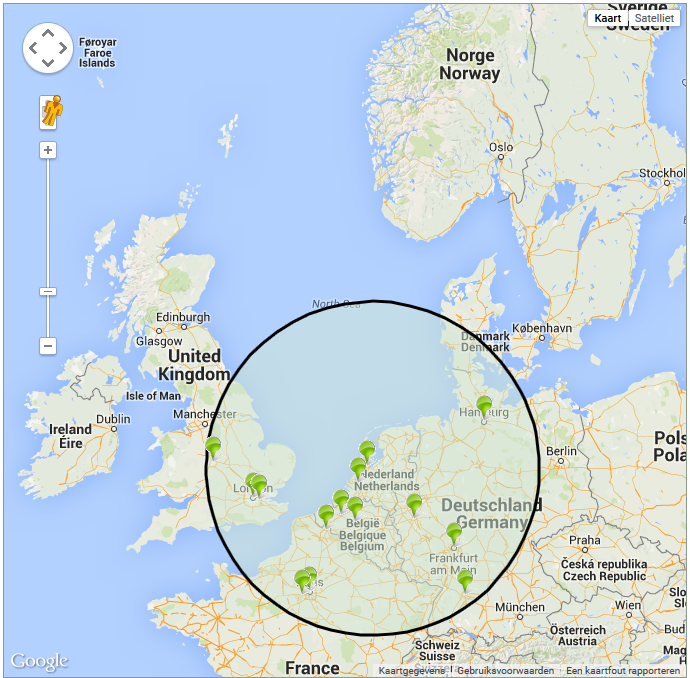
\includegraphics[scale=1.0]{./img/area_w_algo.png}
			\caption{Het zelfde gebied maar nu met het algoritme voor gebiedsrepresentatie}
			\label{fig:with}
		\end{figure}
		\\[0.5cm]
		Een gebied moet dus door een kleiner aantal steden gerepresenteerd worden zodat het aantal zoekopdrachten beperkt blijft en de gebruiker de hoeveelheid nieuws goed kan verwerken. Hiervoor zijn verschillende optie die hieronder besproken zullen worden. Een voorbeeld hiervan is in figuur \ref{fig:with} te zien, dit is het zelfde gebied maar nu met een beperkt aantal steden.
		
		\subsubsection{Aantal steden om een gebied te representeren}
			Het aantal steden om een gebied te representeren is bepaald aan de hand van een gebruikersonderzoek. De opzet en resultaten van dit onderzoek worden bepsroken in sectie \ref{sec:numcities}.
		\subsection{Algoritme 1 - gebiedsrepresentatie}
			Dit algoritme reduceert een lijst steden tot een maximum aantal zodat een gebied goed gerepresenteerd wordt. Dit gaat op de volgende manier:
			\begin{algorithm}
				\caption{Algortime 1 voor gebiedsrepresentatie}
				\mbox{Split():}\\[0.5cm]
				\KwIn{list of cities}
				\KwResult{Reduced list of cities representing the area}
				\mbox{}\\
				\While{number of result $<$ number of cities to represent the area}{
						find biggest city;\\
						add to result;\\
						\mbox{}\\
						\ForEach{city}{
							calculate bearing;\\
							add to corresponding sublist (nw/ne/se/sw);
							}
							\mbox{}\\
						\ForEach{sublist (nw/ne/se/sw)}{
							\eIf{number of cities $<= 5$}{
								find biggest city;\\
								add to result;
								}{
								Split(sublist);\\
								add to result;
								}
							}
					}
			\end{algorithm}\\[0.5cm]
			Dit recursieve algoritme heeft als input een lijst met steden, dit zijn in eerste instantie alle steden die in het door de gebruiker op de kaart geselecteerde gebied liggen. De grootste stad in dit gebied wordt gezocht en aan het eindresultaat toegevoegd. Vervolgens wordt het gebied in vier delen opgedeeld: Noord-Oost, Zuid-Oost, Zuid-West en Noord-West, zie figuur \ref{fig:bearing}. Om deze opdeling te maken wordt voor elke stad de richting, ten opzichte van de grootste stad, berekend (zie algoritme \ref{alg:bearing}) en aan het juiste deel gebied toegevoegd.
			\begin{figure}[!htb]
				\centering
				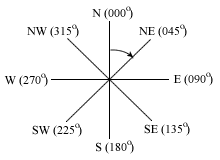
\includegraphics[scale=1.0]{./img/bearings.png}
				\caption{Deelgebieden en hun richting}
				\label{fig:bearing}
			\end{figure}
			\begin{algorithm}
				\caption{Berekenen van de richting}
				\label{alg:bearing}
				\mbox{GetBearing():}\\[0.5cm]
				\KwIn{$(lat_1, lon_1)$, $(lat_2, lon_2)$}
				\KwOut{Bearing in degrees}
				\mbox{}\\
				convert $(lat_1, lon_1)$, $(lat_2, lon_2)$ to radians;\\
				\mbox{}\\
				$\Delta lon = lon_2 - lon_1;$\\
				\mbox{}\\
				$x = \sin(\Delta lon) \cdot \cos(lat_2);$\\
				$y = \cos(lat_1) \cdot \sin(lat_2) - (\sin(lat_1) \cdot \cos(lat_2) \cdot \cos(\Delta lon));$\\
				\mbox{}\\
				$bearing = \arctan(\frac{x}{y});$\\
				\mbox{}\\
				convert bearing to degrees;\\
				\mbox{}\\
				$bearing = \frac{bearing + 360.0}{360.0};$\\
			\end{algorithm}
			Als het aantal steden in een deel gebied kleiner dan of gelijk is aan $5$ wordt de grootste stad in het deelgebied gezocht en aan het eindresultaat toegevoegd. Is het aantal steden echter groter dan wordt het hier boven beschreven proces herhaald voor het deelgebied. \\[0.5cm]
			Aan het einde geeft dit algoritme een lijst van steden die het gebied representeren. Als deze lijst nog steeds meer steden bevat dan het maximale aantal steden om een gebied te representeren wordt dit proces herhaald.
		\subsection{Algoritme 2 - gebiedsrepresentatie}
			Een andere mogelijkheid om een aantal steden die een gebied vertegenwoordigen te selecteren is weer de gootste stad kiezen maar nu het gebied in twee delen splitsen in plaats van vier zoals bij het eerder beschreven algortime.
			\begin{algorithm}
				\caption{Algoritme 2 voor gebiedsrepresentatie}
				\mbox{Split():}\\[0.5cm]
				\KwIn{list of cities}
				\KwResult{Reduced list of cities representing the area}
				\mbox{}\\
				t: list of list of cities;\\
				\mbox{}\\
				\While{number of result $<$ number of cities to represent the area}{
					\ForEach{list in t}{
						\eIf{direction = n/s}{
							biggest, north, south = split\_north(list);\\append biggest to results;\\
							append north, south to t;\\
							remove list from t;\\
							\If{last list in t}{
								set direction to e/w;	
							}	
						}{
						biggest, east, west = split\_east(list);\\append biggest to results;\\
						append north, south to t;\\
						remove list from t;\\
						\If{last list in t}{
							set direction to n/s;	
						}
						}	
					}
				}
			\end{algorithm}\\[0.5cm]
			Het algoritme kiest de grootste stad in het gebied, vevolgens wordt er gekeken welke steden ten noorden liggen en welke steden ten zuiden. Voor elk van deze twee deel gebieden wordt weer de grootste stad gezocht, daarna worden deze deel gebieden opnieuw gesplitst maar nu in oost en west.\\[0.5cm]
			Voor elk deel gebied wordt dus telkens de grootste stad gezocht en deze wordt aan het eindresultaat toegevoegd. het splitsen van een deelgebied gaat om en om: eerst wordt het gebied in noord en zuid gesplitst, dan wordt elk deel gebied in oost en west gesplitst. Nu hebben we vier deelgebieden die allen weer in noord en zuid worden verdeeld etc.
		\subsection{Andere opties}
			Naast deze twee algoritmes zijn er nog enkele andere mogelijkheden om steden te kiezen om een gebied te representeren. Deze werken echter minder goed dan de hier boven beschreven algoritmes.
			\subsubsection{Grootste steden}
				Een mogelijkheid is om alleen de grootste steden in een gebied te selecteren. Voordeel is dat dit een snel en eenvoudig proces is, nadeel is echter dat de verdeling van de grote steden over het gebied (vaak) niet uniform is met als gevolg dat de geselecteerde steden geen goede representatie van het gebied geven.
				%IMAGE
				Een ander probleem bij het selecteren van alleen de grootste steden is dat grote steden, zoals bijvoorbeeld Londen, in meerdere delen in de database staan. Als je nu de grootste steden kiest worden vaak alle drie de delen gekozen met als gevolg dat er clusters ontstaan en er minder steden in de rest van het gebied gekozen kunnen worden.
			\subsubsection{Hoofdsteden}
				In het geval van een selectie van meerdere landen is het een mogelijkheid om alleen de hoofdsteden te gebruiken voor de representatie eventueel aangevuld met de grootste steden in het gebied om voldoende steden te krijgen. Dit is eigenlijk alleen een goede optie als er precies even veel landen als benodigde steden in het gebied liggen. Liggen er minder landen in het gebied, en wordt er aangevuld met de grootste steden, loop je hoogst waarschijnlijk tegen het zelfde probleem aan als wanneer je alleen maar voor de grootste steden kiest. Daarbij komt dat het resultaat vaak nagenoeg gelijk zal zijn omdat hoofdsteden vaak bij de grotere steden horen. 
			\subsubsection{Willekeurig}
				Uit de lijst met steden die in het gebied liggen kunnen willekeurig een aantal steden gekozen worden welke dit gebied representeren. Omdat het hier mogelijk is dat alleen (of grotendeels) kleine/de kleinste steden gekozen worden is dit een minder geschikte mogelijkheid.  Ook is het, net als bij boven genoemde methodes, mogelijk dat de gekozen steden niet verspreid liggen maar zich concentreren in een klein deel van het gebied. Ander groot probleem is dat elke keer dat de gebruiker een gebied selecteert een andere lijst aan steden terug gegeven wordt, hierdoor zullen er elke keer andere nieuws artikelen gezocht worden. Het wordt hierdoor moeilijker (onmogelijk) om een artikel opnieuw op te zoeken met de tool.
		\section{User Interface}
		De User Interface is te zien in figuur \ref{fig:UI}. Aan de linker kant is een kaart te zien waar de gebruiker met de muis een gebied, in de vorm van een cirkel, kan selecteren. Het selecteren van een gebied gaat als volgt:
		\begin{itemize}
			\item Linker muisklik op de kaart waar het middelpunt van het gebied komt
			\item{Ingedrukt houden en slepen, er is nu een groene cirkel te zien}
			\item{Los laten als het gebied de gewenste grootte heeft}
		\end{itemize}
		Aan de rechter kant is een grijs veld waarin een lijst met links naar nieuws artikelen voor het geselecteerde gebied weergegeven wordt.
		\begin{figure}[!htb]
			\centering
			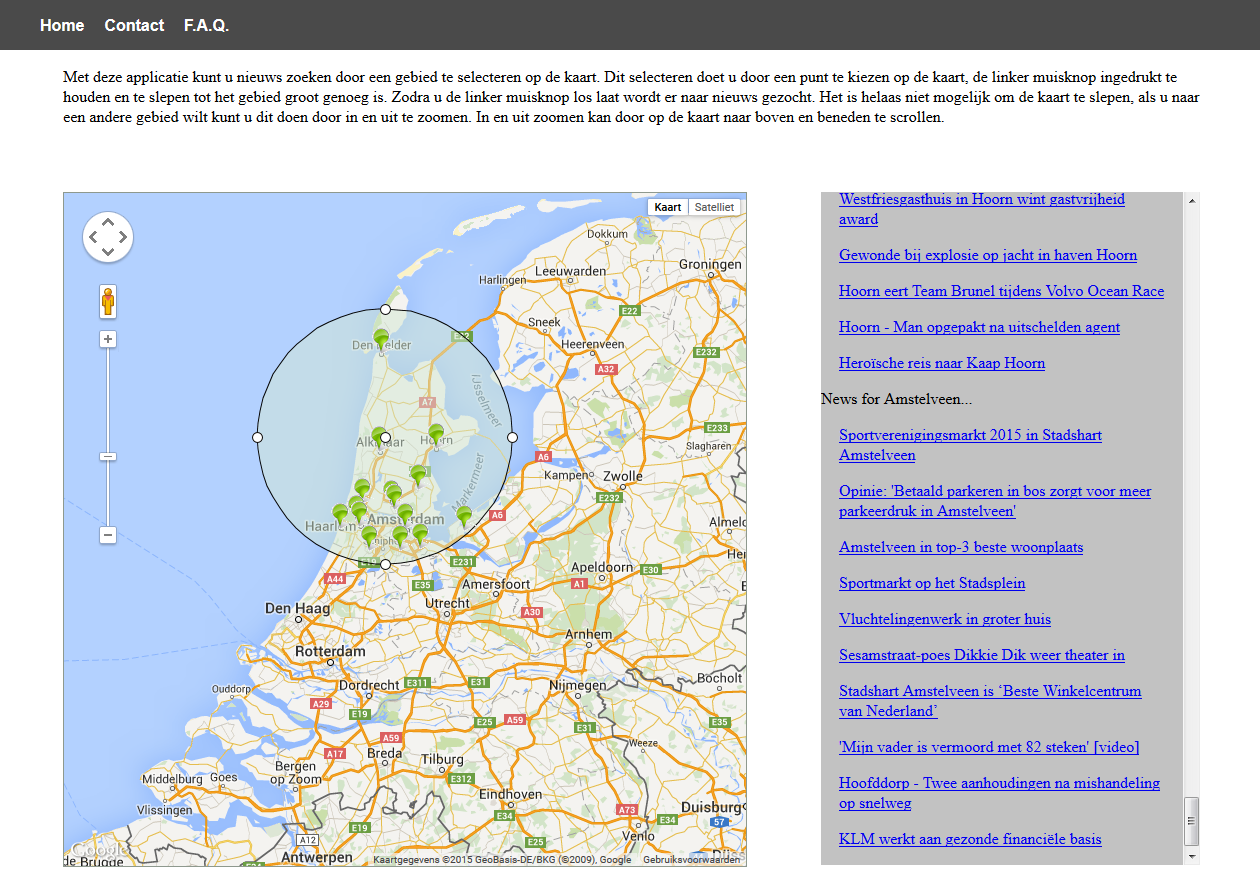
\includegraphics[angle=-90,origin=c,scale=0.70]{./img/UI.png}
			\caption{De User Interface}
			\label{fig:UI}
		\end{figure}
	\section{Samenvatting}
		In dit hoofdstuk hebben we gekeken hoe we het in het voorgaande hoofdstuk voorgestelde ontwerp kunnen implementeren. We hebben gekeken naar PHP, Ruby en Python uiteindelijk hebben we er voor gekozen om de web applicatie met Python, CherryPy en Cheetah te implementeren.
		\\[0.5cm]
		Ook hebben we gekeken hoe we een gebied kunnen representeren met een beperkt aantal steden. Hiervoor hebben we twee algoritmes besproken.
		\\[0.5cm]
		Met dit hoofdstuk hebben we de vragen \textit{Hoe implementeren we een dergelijke applicatie?} en \textit{Kunnen we een gebied representeren door een beperkt aantal steden? En zo ja, hoe?} beantwoord. In het volgende hoofdstuk zullen we de experimenten die uitgevoerd zijn aan de hand van de hier ontwikkelde applicatie bespreken.
\chapter{Experimenten}
	Om te weten of de ontwikkelde applicatie echt een toegevoegde waarde heeft moet er een gebruikers onderzoek uitgevoerd worden. Daarnaast is er een onderzoek nodig om een te bepalen hoeveel steden er nodig zijn om een gebied te representeren, en om een keuze te maken uit de twee voorgestelde algoritmes om deze steden te kiezen. Met deze twee onderzoeken kunnen we de volgende twee vragen beantwoorden:\\[0.5cm]
	\indent \textit{Hoeveel steden zijn er nodig om een gebied te representeren?}
	\\[0.2cm]
	\indent \textit{Wat is de toegevoegde waarde van het zoeken van nieuwsberichten aan de hand van een locatie?}
	\section{Gebiedsrepresentatie}
	\label{sec:numcities}
		Dit onderzoek is gedaan om te bepalen hoeveel steden er nodig zijn om een gebied goed te representeren. Ook wordt er gekeken welke van de twee voorgestelde algoritmes het beste is om de steden te selecteren die het gebied gaan representeren.
		\subsection{Opzet}
			Voor dit experiment is een enqu\^ete gemaakt waarin de gebruiker een afbeelding van een geselecteerd gebied te zien krijgt. Een voorbeeld hiervan wordt gegeven in figuur \ref{fig:area_rep}.
			\begin{figure}[!htb]
				\centering
				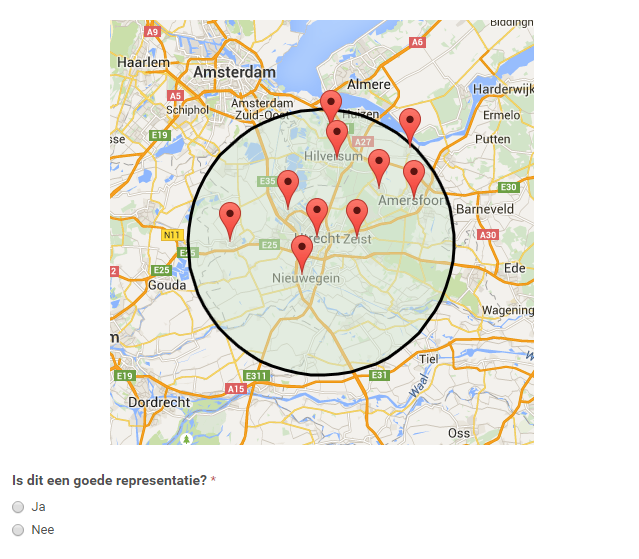
\includegraphics[scale=0.8]{./img/area_rep.png}
				\caption{Voorbeeld vraag gebiedsrepresentatie}
				\label{fig:area_rep}
			\end{figure}
			Bij elke afbeelding krijgt de gebruiker de vraag of dit een goede representatie is van het geselecteerde gebied. Dit is een meerkeuze vraag met als mogelijke antwoorden \textit{ja} en \textit{nee}. Wanneer de gebruiker \textit{nee} kiest krijgt hij of zij een afbeelding van het zelfde gebied te zien maar met meer steden. Er zijn afbeeldingen met tien, vijftien en twintig steden. Zodra er ja gekozen wordt krijgt de gebruiker een vervolg vraag om te bepalen welke van de twee voorgestelde algoritmes beter is. Hiervoor krijgt hij of zij twee afbeeldingen van het zelfde gebied te zien, met het door hem of haar gekozen aantal steden. Een van de afbeeldingen is met algoritme 1 gemaakt terwijl de andere algoritme 2 gebruikt. De vraag is nu welke van de twee representaties beter is, met als mogelijke antwoorden optie 1 of optie 2. Afbeelding \ref{fig:algo} is hier een voorbeeld van. In totaal zijn er voor vier gebebied vragen, dit zijn gebieden met een straal van $25km$, $100km$, $500km$ en $1000km$.
			\\[0.5cm]
			Deze enqu\^ete is in met Google Docs\footnote{http://docs.google.com/} gemaakt en de resultaten worden in een spreadsheet opgeslagen.
			\begin{figure}[!htb]
				\centering
				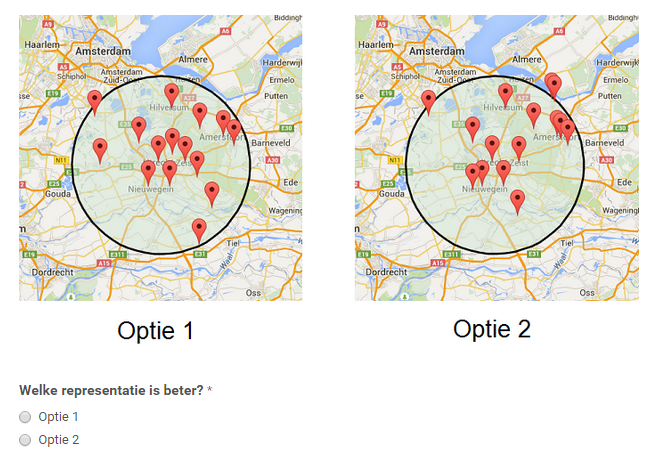
\includegraphics[scale=0.8]{./img/algo.png}
				\caption{Voorbeeld vraag gebiedsrepresentatie}
				\label{fig:algo}
			\end{figure}	
		\newpage		
		\subsection{Resultaten}
			De resultaten zoals deze in het spreadsheet opgeslagen zijn zijn te vinden in bijlage \ref{app:results_rep}. Hier onder worden de resultaten per gebied besproken. De enqu\^ete is door 26 mensen ingevuld met een leeftijd van 15 tot en met 80 jaar. Er zitten ongeveer evenveel mannen als vrouwen in deze groep met allemaal een verschillend opleidingsniveau. Dit is gedaan om een zo goed mogelijk beeld te krijgen van de hoeveelheid steden die nodig is en wat het beste algoritme is.
			\subsubsection{Gebied 1 - straal 25km}
				In tabel \ref{tab:res25} zijn de resultaten te zien voor een gebied met een straal van $25km$. Aan de hand van deze resultaten kunnen we het gemiddelde aantal steden berekenen dat nodig is om dit gebied te representeren: $\frac{11 * 10 + 12 * 15 + 3 * 20}{26} \approx 13.46$ steden. Verder is te zien dat $\frac{24}{26}  * 100\%\approx 92.31\%$ van de respondenten de representatie gegeven door algoritme 1 beter vindt, $\frac{2}{26} * 100\% \approx 7.69\%$ kiest voor algoritme 2.
				\begin{table}[!htb]
					\centering
					\begin{tabular}{| c | c | c | c | c |}
						\hline	
						\textbf{Kandidaat} & \textbf{10 steden} & \textbf{15 steden} & \textbf{20 steden} & \textbf{Algoritme} \\ \hline
						1 & \ding{56} & \ding{52} &  & 1 \\ \hline
						2 & \ding{56} & \ding{52} &  & 1 \\ \hline
						3 & \ding{56} & \ding{52} &  & 1 \\ \hline
						4 & \ding{52} &  &  & 1 \\ \hline
						5 & \ding{52} &  &  & 1 \\ \hline
						6 & \ding{56} & \ding{52} &  & 1 \\ \hline
						7 & \ding{56} & \ding{52} &  & 1 \\ \hline
						8 & \ding{56} & \ding{52} &  & 1 \\ \hline
						9 & \ding{52} &  &  & 1 \\ \hline
						10 & \ding{52} &  &  & 1 \\ \hline
						11 & \ding{52} &  &  & 1 \\ \hline
						12 & \ding{56} & \ding{56} & \ding{52} & 2 \\ \hline
						13 & \ding{52} &  &  & 1 \\ \hline
						14 & \ding{52} &  &  & 1 \\ \hline
						15 & \ding{52} &  &  & 1 \\ \hline
						16 & \ding{56} & \ding{52} &  & 1 \\ \hline
						17 & \ding{52} &  &  & 1 \\ \hline
						18 & \ding{52} &  &  & 1 \\ \hline					
						19 & \ding{56} & \ding{52} &  & 2 \\ \hline
						20 & \ding{56} & \ding{52} &  & 1 \\ \hline
						21 & \ding{56} & \ding{56} & \ding{52} & 1 \\ \hline
						22 & \ding{56} & \ding{52} & & 1 \\ \hline
						23 & \ding{56} & \ding{52} & & 1 \\ \hline
						24 & \ding{56} & \ding{56} & \ding{52} & 1 \\ \hline
						25 & \ding{52} & & & 1 \\ \hline
						26 & \ding{56} & \ding{52} & & 1 \\ \hline
					\end{tabular}
					\caption{Resultaten voor een gebied met straal 25km}
					\label{tab:res25}
				\end{table}
			\subsubsection{Gebied 2 - straal 100km}
				In tabel \ref{tab:res100} zijn de resultaten te zien voor een gebied met een straal van $100km$. Aan de hand van deze resultaten kunnen weer het gemiddelde aantal steden berekenen dat nodig is om dit gebied te representeren: $\frac{8 * 10 + 11 * 15 + 5 * 20}{24} \approx 14.38$ steden. Verder is te zien dat $\frac{23}{26}  * 100\%\approx 88.46\%$ van de respondenten de representatie gegeven door algoritme 1 beter vindt, $\frac{3}{26} * 100\% \approx 11.54\%$ kiest voor algoritme 2. Er is hier bij het berekenen van het gemiddelde aantal steden dat nodig is voor de weergave van dit gebied gedeeld door $24$ omdat twee respondenten geen van de drie representaties goed vonden. Omdat er ook als er op alle drie de vragen nee geantwoord een keuze gemaakt moet worden tussen de twee algoritmes is hier wel door $26$ gedeeld.
				\begin{table}
					\centering
					\begin{tabular}{| c | c | c | c | c |}
						\hline	
						\textbf{Kandidaat} & \textbf{10 steden} & \textbf{15 steden} & \textbf{20 steden} & \textbf{Algoritme} \\ \hline
						1 & \ding{56} & \ding{52} &  & 1 \\ \hline
						2 & \ding{56} & \ding{52} &  & 1 \\ \hline
						3 & \ding{56} & \ding{56} & \ding{52} & 1 \\ \hline
						4 & \ding{56} & \ding{52} &  & 1 \\ \hline
						5 & \ding{56} & \ding{56} & \ding{52} & 1 \\ \hline
						6 & \ding{52} &  &  & 1 \\ \hline
						7 & \ding{56} & \ding{52} &  & 2 \\ \hline
						8 & \ding{52} &  &  & 2 \\ \hline
						9 & \ding{56} & \ding{56} & \ding{56} & 1 \\ \hline
						10 & \ding{52} &  &  & 1 \\ \hline
						11 & \ding{52} &  &  & 1 \\ \hline
						12 & \ding{56} & \ding{56} & \ding{52} & 1 \\ \hline
						13 & \ding{52} &  &  & 1 \\ \hline
						14 & \ding{56} & \ding{56} & \ding{56} & 1 \\ \hline
						15 & \ding{56} & \ding{52} &  & 1 \\ \hline
						16 & \ding{52} &  &  & 1 \\ \hline
						17 & \ding{56} & \ding{52} & & 1 \\ \hline
						18 & \ding{52} &  &  & 2 \\ \hline					
						19 & \ding{56} & \ding{52} &  & 1 \\ \hline
						20 & \ding{56} & \ding{52} &  & 1 \\ \hline
						21 & \ding{56} & \ding{52} &  & 1 \\ \hline
						22 & \ding{56} & \ding{56} & \ding{52} & 1 \\ \hline
						23 & \ding{56} & \ding{56} & \ding{52} & 1 \\ \hline
						24 & \ding{56} & \ding{52} & & 1 \\ \hline
						25 & \ding{52} & & & 1 \\ \hline
						26 & \ding{56} & \ding{52} & & 1 \\ \hline
					\end{tabular}
					\caption{Resultaten voor een gebied met straal 100km}
					\label{tab:res100}
				\end{table}
			\subsubsection{Gebied 3 - straal 500km}
				In tabel \ref{tab:res500} zijn de resultaten te zien voor een gebied met een straal van $500km$. Ook nu weer kunnen we aan an de hand van deze resultaten het gemiddelde aantal steden berekenen dat nodig is om dit gebied te representeren: $\frac{9 * 10 + 14 * 15 + 3 * 20}{26} \approx 13.85$ steden. Verder is te zien dat $\frac{24}{26}  * 100\%\approx 92.31\%$ van de respondenten de representatie gegeven door algoritme 1 beter vindt, $\frac{2}{26} * 100\% \approx 7.69\%$ kiest voor algoritme 2.
				\begin{table}
					\centering
					\begin{tabular}{| c | c | c | c | c |}
						\hline	
						\textbf{Kandidaat} & \textbf{10 steden} & \textbf{15 steden} & \textbf{20 steden} & \textbf{Algoritme} \\ \hline
						1 & \ding{56} & \ding{52} &  & 1 \\ \hline
						2 & \ding{56} & \ding{52} &  & 1 \\ \hline
						3 & \ding{56} & \ding{56} & \ding{52} & 1 \\ \hline
						4 & \ding{56} & \ding{52} &  & 1 \\ \hline
						5 & \ding{56} & \ding{56} & \ding{52} & 1 \\ \hline
						6 & \ding{52} &  &  & 1 \\ \hline
						7 & \ding{56} & \ding{52} &  & 1 \\ \hline
						8 & \ding{52} &  &  & 1 \\ \hline
						9 & \ding{52} &  &  & 1 \\ \hline
						10 & \ding{52} &  &  & 1 \\ \hline
						11 & \ding{56} & \ding{52} &  & 1 \\ \hline
						12 & \ding{56} & \ding{56} & \ding{52} & 1 \\ \hline
						13 & \ding{56} & \ding{52} &  & 1 \\ \hline
						14 & \ding{52} &  &  & 1 \\ \hline
						15 & \ding{56} & \ding{52} &  & 2 \\ \hline
						16 & \ding{56} & \ding{52} &  & 1 \\ \hline
						17 & \ding{52} &  &  & 1 \\ \hline
						18 & \ding{56} & \ding{52} &  & 1 \\ \hline					
						19 & \ding{52} &  &  & 1 \\ \hline
						20 & \ding{52} &  &  & 1 \\ \hline
						21 & \ding{52} &  &  & 1 \\ \hline
						22 & \ding{56} & \ding{52} & & 1 \\ \hline
						23 & \ding{56} & \ding{52} & & 1 \\ \hline
						24 & \ding{56} & \ding{52} & & 2 \\ \hline
						25 & \ding{56} & \ding{52} & & 1 \\ \hline
						26 & \ding{56} & \ding{52} & & 1 \\ \hline
					\end{tabular}
					\caption{Resultaten voor een gebied met straal 500km}
					\label{tab:res500}
				\end{table}
			\subsubsection{Gebied 4 - straal 1000km}
				De resultaten voor een gebied met een straal van $1000km$ zijn te zien in tabel \ref{tab:res1000}. Aan de hand van deze resultaten kunnen we weer het gemiddelde aantal steden berekenen dat nodig is om dit gebied te representeren: $\frac{13 * 10 + 3 * 15 + 9 * 20}{25} \approx 14.20$ steden. Verder is te zien dat $\frac{24}{26}  * 100\%\approx 92.31\%$ van de respondenten de representatie gegeven door algoritme 1 beter vindt, $\frac{2}{26} * 100\% \approx 7.69\%$ kiest voor algoritme 2. Ook hier is door $25$ gedeeld bij de berekening van het gemiddelde aantal steden omdat \'e\'en van de respondenten geen van de drie representaties goed vond.
			\begin{table}
				\centering
				\begin{tabular}{| c | c | c | c | c |}
					\hline	
					\textbf{Kandidaat} & \textbf{10 steden} & \textbf{15 steden} & \textbf{20 steden} & \textbf{Algoritme} \\ \hline
					1 & \ding{56} & \ding{56} & \ding{52} & 1 \\ \hline
					2 & \ding{56} & \ding{52} &  & 1 \\ \hline
					3 & \ding{56} & \ding{56} & \ding{52} & 2 \\ \hline
					4 & \ding{56} & \ding{52} &  & 1 \\ \hline
					5 & \ding{56} & \ding{56} & \ding{52} & 1 \\ \hline
					6 & \ding{52} &  &  & 1 \\ \hline
					7 & \ding{52} &  &  & 1 \\ \hline
					8 & \ding{52} &  &  & 1 \\ \hline
					9 & \ding{52} &  &  & 1 \\ \hline
					10 & \ding{52} &  &  & 1 \\ \hline
					11 & \ding{52} &  &  & 1 \\ \hline
					12 & \ding{56} & \ding{56} & \ding{52} & 1 \\ \hline
					13 & \ding{52} &  &  & 1 \\ \hline
					14 & \ding{52} &  &  & 1 \\ \hline
					15 & \ding{52} &  &  & 1 \\ \hline
					16 & \ding{56} & \ding{56} & \ding{52} & 1 \\ \hline
					17 & \ding{52} &  &  & 1 \\ \hline
					18 & \ding{56} & \ding{56} & \ding{52} & 1 \\ \hline					
					19 & \ding{52} &  &  & 1 \\ \hline
					20 & \ding{52} &  &  & 1 \\ \hline
					21 & \ding{56} & \ding{56} & \ding{52} & 1 \\ \hline
					22 & \ding{56} & \ding{56} & \ding{52} & 1 \\ \hline
					23 & \ding{56} & \ding{56} & \ding{52} & 1 \\ \hline
					24 & \ding{56} & \ding{56} & \ding{56} & 2 \\ \hline
					25 & \ding{52} & & & 1 \\ \hline
					26 & \ding{56} & \ding{52} & & 1 \\ \hline
				\end{tabular}
				\caption{Resultaten voor een gebied met straal 1000km}
				\label{tab:res1000}
			\end{table}
	\section{Toegevoegde waarde}
		Om er achter te komen of de ontwikkelde tool toegevoegde waarde heeft en zo ja wat deze toegevoegde waarde is, is er nog een gebruikersonderzoek gedaan. De opzet en resultaten van dit onderzoek zullen in deze sectie besproken worden.
		\subsection{Opzet}
			Voor dit onderzoek hebben we van te voren een gebieden uitgekozen waar gebruikers naar nieuws moeten zoeken. We hebben de provincie Noord Holland, Nederland uitgekozen. De gebruikers beginnen met het zoeken naar nieuws door gebruik te maken van de traditionele methodes, nieuws sites, websites van kranten en zoekmachines al Google en BING. Hiervoor krijgen de gebruikers vijf minuten waarin ze zoveel mogelijk, voor hen interessant, nieuws proberen te vinden. Na deze vijf minuten krijgen ze de zelfde opdracht maar nu door gebruik te maken van de ontwikkelde tool. Om te kijken of de tool een toegevoegde waarde heeft gaan we kijken hoeveel nieuws de gebruikers in beide situaties hebben kunnen vinden. Daarnaast vragen we de gebruiker ook om feedback. Bij dit onderzoek is er voor gekozen om een zo breed mogelijk doelgroep te nemen. Dit omdat als we bijvoorbeeld alleen ICT studenten nemen de kans groot is dat zij veel beter dan een gemiddeld persoon weten hoe ze zoekopdrachten bij bijvoorbeeld Google uit moeten voeren.
		\subsection{Resultaten}
			De resultaten zoals deze in het spreadsheet opgeslagen zijn zijn te vinden in bijlage \ref{app:results_res}. Hier zullen we deze resulaten bespreken. De enqu\^ete is door 8 mensen ingevuld met een leeftijd van 20 tot 65 jaar. Er zitten ongeveer even veel vrouwen als mannen in deze groep met allemaal een verschillend opleidingsniveau. Dit is gedaan om een zo goed mogelijk beeld te krijgen of en waarom de applicatie een toegevoegde waarde heeft.
			\begin{table}
				\centering
				\begin{tabular}{| c | c | c | c |}
					\hline
					\textbf{Kandidaat} & \textbf{\# artikelen normaal} & \textbf{\# artikelen applicatie} & \textbf{Toegevoegde waarde} \\
					\hline
					1 & 3 & 9 & Ja \\ \hline
					2 & 4 & 5 & Nee \\ \hline
					3 & 5 & 8 & Ja \\ \hline
					4 & 11 & 27 & Ja \\ \hline
					5 & 10 & 25 & Ja \\ \hline
					6 & 4 & 7 & Ja \\ \hline
					7 & 11 & 15 & Ja \\ \hline
					8 & ? & ? & Ja \\ \hline
				\end{tabular}
				\caption{Resultaten onderzoek toegevoegde waarde}
				\label{tab:res}
			\end{table}
			In tabel \ref{tab:res} zien we de resultaten voor dit onderzoek, we zien hier hoeveel nieuws artikelen de respondent in vijf minuten heeft kunnen vinden door gebruik te maken van de al bestaande middelen zoals nieuwssites en Google News (\textit{\# artikelen normaal}), verder zien we de hoeveelheid nieuws artikelen die gevonden zijn door gebruik te maken van de ontwikkelde applicatie (\textit{\# artikelen applicatie}) en we zien of de respondent vindt dat de applicatie toegevoegde waarde heeft. Kandidaat nummer 8 heeft bij \textit{\# artikelen normaal} en \textit{\# artikelen applicatie} een vraagteken staan omdat hier geen aantallen ingevuld zijn. Aan de rest van de resultaten kunnen we zien dat $\frac{7}{8} = 87.50\%$ van de respondenten vindt dat de applicatie een toegevoegde waarde is. Verder zien we dat bij iedereen de hoeveelheid nieuws die ze kunnen vinden in vijf minuten tijd is toegenomen, gemiddeld is deze toename $98.71\%$.
\chapter{Discussie en toekomstig onderzoek}
	\section{Discussie}
	Aan de resultaten van het onderzoek naar de gebiedsrepresentatie is te zien dat het, gemiddeld genomen, niet veel uit maakt. Voor een gebied met een straal van $25km$ zijn gemiddeld $13.46$ steden nodig, voor een groter gebied, met straal $1000km$ is dit gemiddeld $14.20$ steden. Wel is het opvallend dat het gebied met een straal van $100km$ gemiddeld $14.38$ steden nodig heeft. \\[0.5cm]
	Het lijkt er op dat het ideale aantal steden afhangt van de grootte van het gebied, we zien dat bij een gebied met een straal van $25km$ $3$ mensen twintig steden voldoende vinden, bij $100km$ is zijn dit $5$ mensen, maar ook $2$ mensen die geen van de drie geboden representaties voldoende vinden. Kijken we naar een gebied met een straal van $500km$ dan vinden $3$ mensen twintig steden voldoende en bij het grootste gebied, met een straal van $1000km$, zijn dit $9$ mensen en $1$ die geen van de drie representaties goed vindt. Er is dus te zien dat bij een groter gebied meer respondenten voor de representatie met $20$ steden kiezen, al is dit bij een gebied met een straal van $500km$ weer lager. Dit zou kunnen komen omdat het ideale aantal steden niet alleen afhangt van de straal van het gebied maar ook van waar dit gebied gekozen wordt. Om dit te onderzoeken kunnen we de enqu\^ete uitbreiden door meerdere regio's aan te bieden met de zelfde straal.\\[0.5cm]
	In dit onderzoek is ook gekeken welke van de twee voorgestelde algoritmes, zie sectie \ref{sec:rep}, een betere representatie geeft. Bij de gebieden met een straal van $25km$, $500km$ en $1000km$ kiest $92.31\%$ van de respondenten voor algoritme 1, waarbij een gebied steeds in vier delen gesplitst wordt. Bij het gebied met een straal van $100km$ is dit percentage met $88.46\%$ iets lager. We zien dus dat algoritme 1 een beter representatie van een gebied geeft.\\[0.5cm]
	Aan de resultaten van het onderzoek naar de toegevoegde waarde kunnen we zien dat een dergelijke applicatie voor een groot deel, $87.50\%$ een toegevoegde waarde heeft. Wel moet hierbij opgemerkt worden dat de groep respondenten te klein is om een echte conclusie te trekken. Ook zien we dat de hoeveelheid nieuws die in vijf minuten gevonden kan worden bij alle respondenten is toegenomen, hier zijn wel grote verschillen te zien. Deze toename loopt van $25\%$ tot $200\%$. \\[0.5cm]
	We hebben niet alleen gevraagd of de applicatie een toegevoegde waarde heeft maar ook waarom wel of niet. Hoewel de reactie hier natuurlijk veel kunnen verschillen valt op dat $6$ respondenten vinden dat het een toegevoegde waarde heeft omdat ze sneller en eenvoudiger nieuws (uit een regio) kunnen vinden. Van de respondenten vindt \'e\'en dat de applicatie geen toegevoegde waarde heeft omdat er niet op subcategori"en gezocht kan worden, bij andere respondenten zien we dit terug als een van de verbeterpunten. Voor toekomstig onderzoek zou het dus een interessante optie zijn om naast het selecteren van een gebied ook een onderwerp op te kunnen geven. Op deze manier wordt het mogelijk om bijvoorbeeld naar overvallen in Noord Holland te zoeken.
	
	\section{Toekomstig onderzoek}
		Om de applicatie te verbeteren moet er bijvoorbeeld gekeken worden naar het gebruik van andere nieuws bronnen dan zoekmachines en nieuws sites. Denk hierbij aan bijvoorbeeld twitter data, maar ook kan het interessant zijn om naar lokale nieuws bronnen te gaan kijken.
		\subsection{Steden met onbekende populatie}
			\label{sec:citiespop}
			Het probleem van de steden waarvan geen populatie bekend is, zoals beschreven in sectie \ref{sec:geo_info}, is op te lossen door op bijvoorbeeld Wikipedia\footnote{https://en.wikipedia.org/} of WolframAlpha\footnote{http://www.wolframalpha.com/} de populatie op te zoeken. Dit kan gedaan worden door de pagina die over de stad gaat te downloaden en hier vervolgens de populatie uit te halen. We zouden dit kunnen doen op het moment dat een stad geselecteerd worden met populatie $0$, een beter mogelijkheid is waarschijnlijk om dit te doen zodra de database opgebouwd wordt.
		\subsection{Dubbele steden}
			\label{sec:multcities}
			Bij het algoritme voor de gebiedsrepresentatie worden af en toe twee steden heel dicht bij elkaar gekozen, in sommige gevallen gaat dit zelfs om de zelfde stad. Dit komt omdat een aantal grote steden in meerdere delen in de database staan. Een voorbeeld hiervan is \textit{Londen} deze stad staat er als \textit{London} en \textit{City of London} in. Er zijn twee manieren om dit op te lossen.\\[0.5cm]
			Ten eerste kan er gekeken worden of deze steden samen gevoegd kunnen worden. Bij het opbouwen van de database moet dan gekeken worden of er al een stad op dezelfde plek ligt, als dit het geval is wordt de populatie van de tweede stad bij de eerste opgeteld en slaan we dus maar \'e\'en stad op.\\[0.5cm]
			De tweede optie is om het algoritme voor de gebiedsrepresentatie zo aan te passen dat niet twee steden vlak bij elkaar gekozen kunnen worden, ook al zijn dit misschien de grootste steden. Hiervoor moet je voor elke stad die je kiest kijken hoe dicht ze bij de al eerder gekozen steden liggen. Als deze afstand kleiner is dan een minimale afstand moet er een andere stad gekozen worden.
		\subsection{Lokaal nieuws - voorstel}
			\label{sec:localnews}
			Een interessante optie voor de toekomst is om te kijken of het mogelijk is om de nieuwsbronnen af te laten hangen van het geselecteerde gebied, dat wil zeggen dat er gebruik gemaakt wordt van de lokale nieuwsbronnen. Om te bepalen of we te maken hebben met een lokale nieuwsbron kunnen we om te beginnen kijken naar het top-level domain \cite{Toplvl}, ook kan er gekeken worden naar de WHOIS \cite{WHOIS} informatie. Hiermee kan al een aardige schatting gemaakt worden bij welk land de nieuwssite hoort. Om te bepalen bij welke steden de site hoort kunnen we kijken naar bijvoorbeeld de homepage van de nieuwssite. Deze kunnen we analyseren, we kunnen alle namen van steden hier uit halen, als deze grotendeels bij elkaar liggen is de kans groot dat het om een lokale nieuwsbron gaat. Liggen de genoemde steden op de homepage ver uit elkaar, dan is het waarschijnlijk een minder lokale bron.
\chapter{Conclusie}
	Op dit moment is het nog niet (eenvoudig) mogelijk om nieuws te zoeken aan de hand van een locatie, dit zou wel heel nuttig kunnen zijn omdat gebruikers hierdoor een beter begrip van nieuws krijgen. In deze scriptie hebben we gekeken of een applicatie waarmee het mogelijk is om nieuws te zoeken aan de hand van een selectie op een kaart toegevoegde waarde heeft. Om dit te onderzoeken is eerst gekeken hoe we een dergelijke applicatie kunnen opbouwen, er is gekeken welke nieuwsbronnen we kunnen gebruiken en of we een gebied kunnen representeren met een beperkt aantal steden. Voor deze representatie zijn twee algoritmes ontworpen waarvan we de beste aan de hand van een gebruikersonderzoek bepaald hebben.
	\\[0.5cm]
	Het onderzoek naar de gebiedsrepresentatie heeft laten zien dat het aantal steden niet heel veel af hangt van de grootte van een gebied maar dat het ideaal aantal steden wel iets toeneemt naarmate het gebied groter wordt. In het tweede onderzoek is gekeken naar de toegevoegde waarde van de applicatie, hieruit blijkt dat een dergelijke applicatie zeker van toegevoegde waarde kan zijn.
	\\[0.5cm]
	Deze scriptie heeft bewezen dat een applicatie waarmee nieuws gezocht kan worden aan de hand van een locatie van toegevoegde waarde is. Door een gebied op de kaart te selecteren wordt het eenvoudiger en sneller om nieuws uit een bepaalde regio te vinden. Hopelijk wordt er in de toekomst meer onderzoek gedaan naar deze manier van nieuws zoeken zodat dit voor iedereen beschikbaar komt.
	
\begin{thebibliography}{9}
	\bibitem{NewsStand2008} 
	Benjamin E. Teiler, Micheal D. Lieberman, Daniele Panozzo, Jagan Sankaranarayanan, Hanan Samet and Jon Sperling.
	\textit{NewsStand: A New View on News}. 
	In Proceedings of the 16th ACM SIGSPATIAL International Conference on Advances in Geographic Information Systems (ACM GIS 2008), IRVINE, CA, November 2008
	
	\bibitem{STEWARD}
	Micheal D. Lieberman, Hanan Samet, Jagan Sankaranarayanan and Jon Sperling.
	\textit{STEWARD: Architecture of a Spatio-Textual Search Engine}
	15th ACM GIS, Seattle, WA, November 2007
	
	\bibitem{RNwMbESS}
	Hanan Samet, Jagan Sankaranarayanan, Micheal D. Lieberman, Marco D. Adelfio, Brendan C. Fruin, Jack M. Lotkowski, Daniele Panozzo, Jon Sperling and Bejamin E. Teiler.
	\textit{Reading News with Maps by Exploiting Spatial Sysnonyms}
	Communications of the ACM, October 2014
	
	\bibitem{WebAWhere}
	Einat Amitay, Nadav Har'El, Ron Sivan, Aya Soffer.
	\textit{Web-a-Where: Geotagging Web Content}.
	SIGIR'04, July 25-29, 2004, Sheffield, South Yorshire, UK 
	
	\bibitem{TopRes}
	Jochen L. Leidner.
	\textit{Toponym Resolution in Text: ``Which Sheffield is it?''}.
	SIGIR 2004 Sheffield, UK
	
	\bibitem{GeoDist}
	Wikipedia.
	\textit{Geographical distance}
	URL: \url{https://en.wikipedia.org/wiki/Geographical_distance}
	(april 2015)
	
	\bibitem{FinPoi}
	Jan Philip Matuschek. \textit{Finding Points Within a Distance of a Latitude/Longitude Using Bounding Coordinates}. 
	URL: \url{http://janmatuschek.de/LatitudeLongitudeBoundingCoordinates}
	(april 2015)
	
	\bibitem{CalDist}
	Movable Type Scripts. \textit{Calculate distance, bearing and more between Latitude/Longitude points}. 
	URL: \url{http://www.movable-type.co.uk/scripts/latlong.html}
	(april 2015)
	
	\bibitem{MapsJS}
	Google. 
	\textit{Google Maps JavaScript API }. 
	URL: 
\url{	https://developers.google.com/maps/documentation/
	javascript/tutorial}
	(april 2015)
	
	\bibitem{NewsAPI}
	Google.
	\textit{News Search (Deprecated)}.
	URL: \url{https://developers.google.com/news-search/}
	(mei 2015)
	
	\bibitem{BINGNews}
	BING. 
	\textit{Bing Search API}.
	URL: \url{http://datamarket.azure.com/dataset/bing/search}
	(mei 2015)
	
	\bibitem{YahooNews}
	Yahoo.
	\textit{News Service}.
	URL: \url{https://developer.yahoo.com/boss/search/boss_api_guide/news.html}
	(mei 2015)
	
	\bibitem{Faroo}
	Faroo.
	\textit{Free API}.
	URL: \url{http://www.faroo.com/hp/api/api.html}
	(mei 2015)
	
	\bibitem{SQLite}
	\textit{SQLite}. 
	URL: \url{https://www.sqlite.org/}
	(april 2015)
	
	\bibitem{LauScr}
	Laurens Verspeek. 
	\textit{Trusting websites using geo-graphical consistency}.
	June 20, 2014
	
	\bibitem{CherryPy}
	Python.
	\textit{CherryPy}.
	URL: \url{http://www.cherrypy.org/}
	(april 2015)
	
	\bibitem{Cheetah}
	Python.
	\textit{Cheetah}.
	URL: \url{http://www.cheetahtemplate.org/}
	(april 2015)
	
	\bibitem{JSON}
	\textit{JSON}.
	URL: \url{http://json.org/}
	(april 2015)
	
	\bibitem{AJAX}
	\textit{AJAX}.
	URL: \url{http://en.wikipedia.org/wiki/Ajax_(programming)}
	(april 2015)
	
	\bibitem{Geonames}
	\textit{Geonames}.
	URL: \url{http://www.geonames.org/}
	(april 2015)
	
	\bibitem{JQuery}
	\textit{JQuery}.
	URL: \url{https://jquery.com/}
	(april 2015)
	
	\bibitem{RSS}
	\textit{RSS Feeds}.
	URL: \url{http://en.wikipedia.org/wiki/RSS}
	(mei 2015)
	
	\bibitem{sqlite3}
	Python.
	\textit{sqlite3}.
	URL: \url{https://docs.python.org/2/library/sqlite3.html}
	(april 2015)
	
	\bibitem{zipfile}
	Python.
	\textit{zipfile}.
	URL: \url{https://docs.python.org/2/library/zipfile.html}
	(april 2015)
	
	\bibitem{urllib2}
	Python.
	\textit{urllib2}.
	URL: \url{https://docs.python.org/2/library/urllib2.html}
	(april 2015)
	
	\bibitem{spherical}
	Wikipedia.
	\textit{Spherical law of cosines}.
	URL: \url{https://en.wikipedia.org/wiki/Spherical_law_of_cosines}
	(april 2015)
	
	\bibitem{haversine}
	Wikipedia.
	\textit{Haversine Formula}.
	URL: \url{https://en.wikipedia.org/wiki/Haversine_formula}
	(april 2015)
	
	\bibitem{circlelat}
	Wikipedia.
	\textit{Circle of latitude}.
	URL: \url{https://en.wikipedia.org/wiki/Circle_of_latitude}
	(april 2015)
	
	\bibitem{circlesphere}
	Wikipedia.
	\textit{Circle of a sphere}.
	URL: \url{https://en.wikipedia.org/wiki/Circle_of_a_sphere}
	(april 2015)
	
	\bibitem{greatcircle}
	Wikipedia.
	\textit{Great circle}.
	URL: \url{https://en.wikipedia.org/wiki/Great_circle}
	(april 2015)
	
	\bibitem{Wolf}
	\textit{WolframAlpha}.
	URL: \url{http://www.wolframalpha.com/}
	(april 2015)
	
	\bibitem{HTTP}
	Wikipedia.
	\textit{Hypertext Transfer Protocol}.
	URL: \url{http://en.wikipedia.org/wiki/Hypertext_Transfer_Protocol}
	(mei 2015)
	
	\bibitem{API}
	Wikipedia.
	\textit{Application programming interface}.
	URL: \url{http://en.wikipedia.org/wiki/Application_programming_interface}
	(mei 2015)
	
	\bibitem{SQL}
	Wikipedia.
	\textit{SQL}.
	URL: \url{http://en.wikipedia.org/wiki/SQL}
	(april 2015)
	
	\bibitem{Pytha}
	Wikipedia.
	\textit{Pythagorean theorem}.
	URL: \url{http://en.wikipedia.org/wiki/Pythagorean_theorem}
	(april 2015)
	
	\bibitem{WHOIS}
	Wikipedia.
	\textit{WHOIS}.
	URL: \url{https://en.wikipedia.org/wiki/WHOIS}
	(juni 2015)
	
	\bibitem{Toplvl}
	Wikipedia.
	\textit{Domain name, Top-level domains}
	URL: \url{https://en.wikipedia.org/wiki/Domain_name#Top-level_domains}
	(juni 2015)
	
	\bibitem{Mathbook}
	W. Gellert, S. Gottwald, M. Hellwich, H. Kästner, and H. Küstner. 
	\textit{The VNR Concise Encyclopedia of Mathematics}.
	 2nd ed., ch. 12 (Van Nostrand Reinhold: New York, 1989).
\end{thebibliography}
\newpage
\appendix
\chapter{Installatie}
	\label{app:install}
	\section{Systeem vereisten}
		\begin{itemize}
			\item Linux server (bijvoorbeeld Ubuntu Server)
			\item Python 2.7
			\item CherryPy
			\item Cheetah
			\item sqlite3 (Python module)
			\item SQLite
			\item Minimaal $7MB$ vrije ruimte op HDD
		\end{itemize}
	\section{Toevoegen extensies aan SQLite}
		Om extensies aan SQLite toe te kunnen voegen moeten we eerste het pakket \textit{libsqlite3-dev} installeren. Op een Ubuntu Server gaat dat als volgt:
		\begin{verbatim}
		sudo apt-get install libsqlite3-dev
		\end{verbatim}
		Vervolgens moeten we het C bestand met de extensie compileren:
		\begin{verbatim}
		gcc -fPIC -lm -shared extension-functions.c -o libsqlitefunctions.so
		\end{verbatim}
	\section{Server installatie}
		Om de server te installeren moeten we deze downloaden van de volgende link:
		\begin{verbatim}
		https://github.com/thomasvanophem/Afstudeerproject/tree/master/Source/Server
		\end{verbatim}
		Deze bestanden moeten allemaal in de zelfde map op de server geplaatst worden.
	\section{Server starten}
		De server starten gaat met het volgende commando:
		\begin{verbatim}
		python server.py
		\end{verbatim}
		De server wordt opgestart en is nu te vinden via http://$<$ip adres server$>$:8080, bijvoorbeeld:
		\begin{verbatim}
		http://192.168.0.13:8080
		\end{verbatim}
		De eerste keer dat de server gestart wordt moet de database opgebouwd worden, dit gebeurt door de variable \textit{download} in \textit{config.py} op \textit{True} te zetten. Het is aan te raden om hierna deze variable op \textit{False} te zetten zodat de database niet elke keer opgebouwd wordt als de server herstart wordt.
\chapter{Resultaten onderzoek gebiedsrepresentatie}
\label{app:results_rep}

\begin{sidewaystable}
	\centering
	\caption{Resultaten onderzoek gebiedsrepresentatie}
	\begin{tabular}{|l|l|l|l|l|l|l|l|l|l|l|l|l|l|l|l|l|l|l|}
		\hline
		{\bf 10} & {\bf 15} & {\bf 20} & {\bf 1 or 2} & {\bf 10} & {\bf 15} & {\bf 20} & {\bf 1 or 2} & {\bf 10} & {\bf 15} & {\bf 20} & {\bf 1 or 2} & {\bf 10} & {\bf 15} & {\bf 20} & {\bf 1 or 2} & {\bf age} & {\bf sex} & {\bf level}   \\  \hline
		Nee      & Ja       &          & Optie 1                             & Nee      & Ja       &          & Optie 1                             & Nee      & Ja       &          & Optie 1                             & Nee      & Nee      & Ja       & Optie 1                             &                    &                    &                                                          \\  \hline
		Nee      & Ja       &          & Optie 1                             & Nee      & Ja       &          & Optie 1                             & Nee      & Ja       &          & Optie 1                             & Nee      & Ja       &          & Optie 1                             &                    &                    &                                                          \\  \hline
		Nee      & Ja       &          & Optie 1                             & Nee      & Nee      & Ja       & Optie 1                             & Nee      & Nee      & Ja       & Optie 1                             & Nee      & Nee      & Ja       & Optie 2                             &                    &                    &                                                         \\  \hline
		Ja       &          &          & Optie 1                             & Nee      & Ja       &          & Optie 1                             & Nee      & Ja       &          & Optie 1                             & Nee      & Ja       &          & Optie 1                             &                    &                    &                                                          \\  \hline
		Ja       &          &          & Optie 1                             & Nee      & Nee      & Ja       & Optie 1                             & Nee      & Nee      & Ja       & Optie 1                             & Nee      & Nee      & Ja       & Optie 1                             &                    &                    &                                                          \\  \hline
		Nee      & Ja       &          & Optie 1                             & Ja       &          &          & Optie 1                             & Ja       &          &          & Optie 1                             & Ja       &          &          & Optie 1                             &                    &                    &                                                          \\  \hline
		Nee      & Ja       &          & Optie 1                             & Nee      & Ja       &          & Optie 2                             & Nee      & Ja       &          & Optie 1                             & Ja       &          &          & Optie 1                             &                    &                    &                                                          \\  \hline
		Nee      & Ja       &          & Optie 1                             & Ja       &          &          & Optie 2                             & Ja       &          &          & Optie 1                             & Ja       &          &          & Optie 1                             &                    &                    &                                                          \\  \hline
		Ja       &          &          & Optie 2                             & Nee      & Nee      & Nee      & Optie 1                             & Ja       &          &          & Optie 1                             & Ja       &          &          & Optie 1                             &                    &                    &                                                          \\  \hline
		Ja       &          &          & Optie 2                             & Ja       &          &          & Optie 1                             & Ja       &          &          & Optie 1                             & Ja       &          &          & Optie 1                             &                    &                    &                                                          \\  \hline
		Ja       &          &          & Optie 2                             & Ja       &          &          & Optie 1                             & Nee      & Ja       &          & Optie 1                             & Ja       &          &          & Optie 1                             &                    &                    &                                                          \\  \hline
		Nee      & Nee      & Ja       & Optie 2                             & Nee      & Nee      & Ja       & Optie 1                             & Nee      & Nee      & Ja       & Optie 1                             & Nee      & Nee      & Ja       & Optie 1                             &                    &                    &                                                          \\  \hline
		Ja       &          &          & Optie 1                             & Ja       &          &          & Optie 1                             & Nee      & Ja       &          & Optie 1                             & Ja       &          &          & Optie 1                             &                    &                    &                                                         \\  \hline
		Ja       &          &          & Optie 1                             & Nee      & Nee      & Nee      & Optie 1                             & Ja       &          &          & Optie 1                             & Ja       &          &          & Optie 1                             &                    &                    &                                                          \\  \hline
		Ja       &          &          & Optie 1                             & Nee      & Ja       &          & Optie 1                             & Nee      & Ja       &          & Optie 2                             & Ja       &          &          & Optie 1                             &                    &                    &                                                         \\  \hline
		Nee      & Ja       &          & Optie 1                             & Ja       &          &          & Optie 1                             & Nee      & Ja       &          & Optie 1                             & Nee      & Nee      & Ja       & Optie 1                             &                    &                    &                                                          \\  \hline
		Ja       &          &          & Optie 1                             & Nee      & Ja       &          & Optie 1                             & Ja       &          &          & Optie 1                             & Ja       &          &          & Optie 1                             &                    &                    &                                                          \\  \hline
		Ja       &          &          & Optie 1                             & Ja       &          &          & Optie 2                             & Nee      & Ja       &          & Optie 1                             & Nee      & Nee      & Ja       & Optie 1                             &                    &                    &                                                          \\  \hline
		Nee      & Ja       &          & Optie 2                             & Nee      & Ja       &          & Optie 1                             & Ja       &          &          & Optie 1                             & Ja       &          &          & Optie 1                             &                    &                    &                                                        \\  \hline
		Nee      & Ja       &          & Optie 1                             & Nee      & Ja       &          & Optie 1                             & Ja       &          &          & Optie 1                             & Ja       &          &          & Optie 1                             &                    &                    &                                                         \\  \hline
		Nee      & Nee      & Ja       & Optie 1                             & Nee      & Ja       &          & Optie 1                             & Ja       &          &          & Optie 1                             & Nee      & Nee      & Ja       & Optie 1                             &                    &                    &                                                         \\  \hline
		Nee      & Ja       &          & Optie 1                             & Nee      & Nee      & Ja       & Optie 1                             & Nee      & Ja       &          & Optie 1                             & Nee      & Nee      & Ja       & Optie 1                             & 22                 & Man                &                             WO                           \\  \hline
		Nee      & Ja       &          & Optie 1                             & Nee      & Nee      & Ja       & Optie 1                             & Nee      & Ja       &          & Optie 1                             & Nee      & Nee      & Ja       & Optie 1                             & 26                 & Man                &                             MBO                          \\  \hline
		Nee      & Nee      & Ja       & Optie 1                             & Nee      & Ja       &          & Optie 1                             & Nee      & Ja       &          & Optie 2                             & Nee      & Nee      & Nee      & Optie 2                             & 67                 & Man                &                             MBO                         \\  \hline
		Ja       &          &          & Optie 1                             & Ja       &          &          & Optie 1                             & Nee      & Ja       &          & Optie 1                             & Ja       &          &          & Optie 1                             &                    &                    &                                                        \\  \hline
		Nee      & Ja       &          & Optie 1                             & Nee      & Ja       &          & Optie 1                             & Nee      & Ja       &          & Optie 1                             & Nee      & Ja       &          & Optie 1                             & 49                 & Man                &                             HBO                          \\  \hline
	\end{tabular}
\end{sidewaystable}
\chapter{Resultaten onderzoek toegevoegde waarde}
\label{app:results_res}
\begin{table}
	\centering
	\begin{tabular}{|l|l|}
		\hline
		\textbf{sex} & Man \\ \hline
		\textbf{age} & 22 \\ \hline
		\textbf{level} & WO \\ \hline
		\textbf{\# normal} & 3 \\ \hline
		\textbf{sources} & Noord Hollands Dagblad \\ \hline
		\textbf{\# application} & 9 \\ \hline
		\textbf{added value} & Ja \\ \hline
		\textbf{why} & Makkelijk en sneller om nieuws te vinden.
		Een duidelijk overzicht\\ \hline
		
		\textbf{improvements} & Ook de mogelijkheid bieden om een onderwerp op te geven. \\ \hline
	\end{tabular}
\end{table}
\begin{table}
	\centering
	\begin{tabular}{|l|l|}
		\hline
		\textbf{sex} & Vrouw \\ \hline
		\textbf{age} & 18 \\ \hline
		\textbf{level} & MBO \\ \hline
		\textbf{\# normal} & 4 \\ \hline
		\textbf{sources} & Google, dichtbij
		 \\ \hline
		\textbf{\# application} & 5 \\ \hline
		\textbf{added value} & Nee \\ \hline
		\textbf{why} & Hij gaat niet op subcategorie"en. \\ \hline
		\textbf{improvements} & Via de telefoon werk hij niet zo snel.
		Layout kan iets mooier
		 \\ \hline
	\end{tabular}
\end{table}
\begin{table}
	\centering
	\begin{tabular}{|l|l|}
		\hline
		\textbf{sex} & Man \\ \hline
		\textbf{age} & 61 \\ \hline
		\textbf{level} & Voortgezet onderwijs \\ \hline
		\textbf{\# normal} & 5 \\ \hline
		\textbf{sources} & Telegraaf noordhollands dagblad nieuws .nl
		 \\ \hline
		\textbf{\# application} & 8 \\ \hline
		\textbf{added value} & Ja \\ \hline
		\textbf{why} & \pbox{20cm}{regio selectie per plaats naam uitzoeken \\sneller over zicht van het nieuws 
		\\door korte inhoud z.g koppensnellen hierdoor voor mij interessanten nieuws}
		\\ \hline
		
		\textbf{improvements} & Is het mogelijk op onder werp te zoeken?
		 \\ \hline
	\end{tabular}
\end{table}
\begin{table}
	\centering
	\begin{tabular}{|l|l|}
		\hline
		\textbf{sex} & Man \\ \hline
		\textbf{age} & 23 \\ \hline
		\textbf{level} & WO \\ \hline
		\textbf{\# normal} & 11 \\ \hline
		\textbf{sources} & Google news
		rtvnh.nl
		noordhollandsdagblad.nl
		dichtbij.nl
		nu.nl
		parool.nl
		
		\\ \hline
		\textbf{\# application} & 27 \\ \hline
		\textbf{added value} & Ja \\ \hline
		\textbf{why} & Eenvoudig en snel nieuws vinden uit een regio
		overzichtelijk weergegeven
		
		\\ \hline
		
		\textbf{improvements} & \pbox{20cm}{Zoeken op onderwerp (dus gebied selecteren maar ook onderwerp,\\ bijvoorbeeld; schietpartij noord holland}
		
		\\ \hline
	\end{tabular}
\end{table}
\begin{table}
	\centering
	\begin{tabular}{|l|l|}
		\hline
		\textbf{sex} & Vrouw \\ \hline
		\textbf{age} & 54 \\ \hline
		\textbf{level} & HBO \\ \hline
		\textbf{\# normal} & 10 \\ \hline
		\textbf{sources} & Noord hollands dagblad, Nu.nl
		\\ \hline
		\textbf{\# application} & 25 \\ \hline
		\textbf{added value} & Ja \\ \hline
		\textbf{why} & verzameling onderwerpen staat handig onder elkaar vermeld.
		
		
		\\ \hline
		
		\textbf{improvements} & bronvermelding bij onderwerp.
		datum van artikel.
		
		
		\\ \hline
	\end{tabular}
\end{table}
\begin{table}
	\centering
	\begin{tabular}{|l|l|}
		\hline
		\textbf{sex} & Man \\ \hline
		\textbf{age} & 25 \\ \hline
		\textbf{level} & WO \\ \hline
		\textbf{\# normal} & 4 \\ \hline
		\textbf{sources} & google news, rtvnh.nl
		\\ \hline
		\textbf{\# application} & 7 \\ \hline
		\textbf{added value} & Ja \\ \hline
		\textbf{why} & \pbox{20cm}{Het nieuws is accurater en de applicatie verzamelt\\ berichten uit een groot aantal bronnen.
		\\Het is makkelijk om een snel een overzicht te krijgen van al het \\nieuws uit een regio.}
		
		
		
		\\ \hline
		
		\textbf{improvements} & \pbox{20cm}{De manier van het selecteren van een regio zou makkelijker kunnen. \\ Het bewegen over de kaart en het slepen om een cirkel te vormen is niet 100\% intuitief.}
		
		
		
		\\ \hline
	\end{tabular}
\end{table}
\begin{table}
	\centering
	\begin{tabular}{|l|l|}
		\hline
		\textbf{sex} & Man \\ \hline
		\textbf{age} & 22 \\ \hline
		\textbf{level} & WO \\ \hline
		\textbf{\# normal} & 11 \\ \hline
		\textbf{sources} & google news, rtvnh.nl
		\\ \hline
		\textbf{\# application} & 15 \\ \hline
		\textbf{added value} & Ja \\ \hline
		\textbf{why} & \pbox{20cm}{Een handige manier om lokaal nieuws op te zoeken,\\ zonder daarvoor verschillende nieuwswebsites te hoeven bekijken.\\ Een voordeel is dat de applicatie snel reageert op een nieuw geselecteerd gebied, \\dat draagt bij aan het gebruiksgemak en de totale ervaring.}
		
		
		
		
		\\ \hline
		
		\textbf{improvements} & \pbox{20cm}{- Mogelijk maken om huidige selectie aan te passen \\- nu wordt direct een nieuwe selectie getekend.
		\\- Preview van nieuwsitems weergeven in het nieuwsoverzicht aan de rechterkant.
		\\- Afbeeldingen bij nieuwsberichten ophalen en tonen in het nieuwsoverzicht\\ (als het bericht een afbeelding bevat).
		\\- Melding geven als er geen nieuwsberichten zijn gevonden.
		}
		
		
		
		\\ \hline
	\end{tabular}
\end{table}
\begin{table}
	\centering
	\begin{tabular}{|l|l|}
		\hline
		\textbf{sex} & Vrouw \\ \hline
		\textbf{age} & 23 \\ \hline
		\textbf{level} & MBO \\ \hline
		\textbf{\# normal} & ? \\ \hline
		\textbf{sources} & Telegraaf 
		
		\\ \hline
		\textbf{\# application} & ? \\ \hline
		\textbf{added value} & Ja \\ \hline
		\textbf{why} & \pbox{20cm}{Ik snap er niks van van de onderzoek...\\
			Als ik het goed begrijp word er onderzocht wat voor nieuws de mensen\\ meer aanspreken onder bepaalde leeftijden."
			}
		
		
		
		
		\\ \hline
		
		\textbf{improvements} & \pbox{20cm}{Duidelijkheid waar dit precies over gaat}
			
		
		
		
		\\ \hline
	\end{tabular}
\end{table}
\end{document}